% !TeX spellcheck = russian-aot-ieyo
% Зачем: Определяет класс документа (То, как будет выглядеть документ)
% Примечание: параметр draft помечает строки, вышедшие за границы страницы, прямоугольником, в фильной версии его нужно удалить.
\documentclass[a4paper,14pt,russian,oneside,final]{extreport}

% Зачем: Предоставляет проприетарный Times New Roman.
% ОБНОВЛЕНИЕ: лучше использовать scalable-cyrfonts-tex: меньше проблем с установкой
% Из руководства к PSCyr: "Во избежание проблем пакет PSCyr должен загружаться перед пакета-ми inputenc и babel".
% Примечание: Требует шаманства при установке, инструкция http://plumbum-blog.blogspot.com/2010/06/miktex-28-pscyr-04d.html
% http://blog.harrix.org/?p=444
% надо закомментировать это, чтобы использовать scalable-cyrfonts-tex:
\usepackage{pscyr}
\let\Tiny=\tiny

% Зачем: Предоставляет свободный Times New Roman.
% Шрифт идёт вместе с пакетом scalable-cyrfonts-tex в Ubuntu/Debian
% раскомментировать, чтобы использовать scalable-cyrfonts-tex:
%\usefont{T2A}{ftm}{m}{sl}


% Зачем: Установка кодировки исходных файлов.
\usepackage[utf8]{inputenc}

% Зачем: Делает результирующий PDF "searchable and copyable".
\usepackage{cmap}

% Зачем: Выбор внутренней TeX кодировки.
\usepackage[T2A]{fontenc}

% Зачем: Чтобы можно было использовать русские буквы в формулах, но в случае использования предупреждать об этом.
\usepackage[warn]{mathtext}

% Зачем: Учет особенностей различных языков.
\usepackage[russian]{babel}

% Зачем: Добавляет поддержу дополнительных размеров текста 8pt, 9pt, 10pt, 11pt, 12pt, 14pt, 17pt, and 20pt.
% Почему: Пункт 2.1.1 Требований по оформлению пояснительной записки.
\usepackage{extsizes}


% Зачем: Длинна, пимерно соответвующая 5 символам
% Почему: Требования содержат странное требование про отсупы в 5 символов (для немоноширинного шрифта :| )
\newlength{\fivecharsapprox}
\setlength{\fivecharsapprox}{6ex}


% Зачем: Добавляет отступы для абзацев.
% Почему: Пункт 2.1.3 Требований по оформлению пояснительной записки.
\usepackage{indentfirst}
\setlength{\parindent}{\fivecharsapprox} % Примерно соответсвует 5 символам.


% Зачем: Настраивает отступы от границ страницы.
% Почему: Пункт 2.1.2 Требований по оформлению пояснительной записки.
\usepackage[left=3cm,top=2.0cm,right=1.5cm,bottom=2.7cm]{geometry}


% Зачем: Настраивает межстрочный интервал, для размещения 40 +/- 3 строки текста на странице.
% Почему: Пункт 2.1.1 Требований по оформлению пояснительной записки.
\usepackage[nodisplayskipstretch]{setspace}
\setstretch{1.1}
%\onehalfspacing

% Зачем: Выбор шрифта по-умолчанию.
% Почему: Пункт 2.1.1 Требований по оформлению пояснительной записки.
% Примечание: В требованиях не указан, какой именно шрифт использовать. По традиции используем TNR.
\renewcommand{\rmdefault}{ftm} % Times New Roman


% Зачем: Отключает использование изменяемых межсловных пробелов.
% Почему: Так не принято делать в текстах на русском языке.
\frenchspacing


% Зачем: Сброс счетчика сносок для каждой страницы
% Примечание: в "Требованиях по оформлению пояснительной записки" не указано, как нужно делать, но в других БГУИРовских докуметах рекомендуется нумерация отдельная для каждой страницы
\usepackage{perpage}
\MakePerPage{footnote}


% Зачем: Добавляет скобку 1) к номеру сноски
% Почему: Пункты 2.9.2 и 2.9.1 Требований по оформлению пояснительной записки.
\makeatletter
\def\@makefnmark{\hbox{\@textsuperscript{\normalfont\@thefnmark)}}}
\makeatother


% Зачем: Расположение сносок внизу страницы
% Почему: Пункт 2.9.2 Требований по оформлению пояснительной записки.
\usepackage[bottom]{footmisc}


% Зачем: Переопределяем стандартную нумерацию, т.к. в отчете будут только section и т.д. в терминологии TeX
\makeatletter
\renewcommand{\thesection}{\arabic{section}}
\makeatother


% Зачем: Пункты (в терминологии требований) в терминологии TeX subsubsection должны нумероваться
% Почему: Пункт 2.2.3 Требований по оформлению пояснительной записки.
\setcounter{secnumdepth}{3}


% Зачем: Настраивает отступ между таблицей с содержанимем и словом СОДЕРЖАНИЕ
% Почему: Пункт 2.2.7 Требований по оформлению пояснительной записки.
\usepackage{tocloft}
\setlength{\cftbeforetoctitleskip}{-1em}
\setlength{\cftaftertoctitleskip}{1em}


% Зачем: Определяет отступы слева для записей в таблице содержания.
% Почему: Пункт 2.2.7 Требований по оформлению пояснительной записки.
\makeatletter
\renewcommand{\l@section}{\@dottedtocline{1}{0.5em}{1.2em}}
\renewcommand{\l@subsection}{\@dottedtocline{2}{1.7em}{2.0em}}
\makeatother


% Зачем: Работа с колонтитулами
\usepackage{fancyhdr} % пакет для установки колонтитулов
\pagestyle{fancy} % смена стиля оформления страниц


% Зачем: Нумерация страниц располагается справа снизу страницы
% Почему: Пункт 2.2.8 Требований по оформлению пояснительной записки.
\fancyhf{} % очистка текущих значений
\fancyfoot[R]{\thepage} % установка верхнего колонтитула
\renewcommand{\footrulewidth}{0pt} % убрать разделительную линию внизу страницы
\renewcommand{\headrulewidth}{0pt} % убрать разделительную линию вверху страницы
\fancypagestyle{plain}{
    \fancyhf{}
    \rfoot{\thepage}}


% Зачем: Задает стиль заголовков раздела жирным шрифтом, прописными буквами, без точки в конце
% Почему: Пункты 2.1.1, 2.2.5, 2.2.6 и ПРИЛОЖЕНИЕ Л Требований по оформлению пояснительной записки.
\makeatletter
\renewcommand\section{%
  \clearpage\@startsection {section}{1}%
    {\fivecharsapprox}%
    {-1em \@plus -1ex \@minus -.2ex}%
    {1em \@plus .2ex}%
    {\raggedright\hyphenpenalty=10000\normalfont\large\bfseries\MakeUppercase}}
\makeatother


% Зачем: Задает стиль заголовков подразделов
% Почему: Пункты 2.1.1, 2.2.5 и ПРИЛОЖЕНИЕ Л Требований по оформлению пояснительной записки.
\makeatletter
\renewcommand\subsection{%
  \@startsection{subsection}{2}%
    {\fivecharsapprox}%
    {-1em \@plus -1ex \@minus -.2ex}%
    {1em \@plus .2ex}%
    {\raggedright\hyphenpenalty=10000\normalfont\normalsize\bfseries}}
\makeatother


% Зачем: Задает стиль заголовков пунктов
% Почему: Пункты 2.1.1, 2.2.5 и ПРИЛОЖЕНИЕ Л Требований по оформлению пояснительной записки.
\makeatletter
\renewcommand\subsubsection{
  \@startsection{subsubsection}{3}%
    {\fivecharsapprox}%
    {-1em \@plus -1ex \@minus -.2ex}%
    {\z@}%
    {\raggedright\hyphenpenalty=10000\normalfont\normalsize\bfseries}}
\makeatother

% Зачем: для оформления введения и заключения, они должны быть выровнены по центру.
% Почему: Пункты 1.1.15 и 1.1.11 Требований по оформлению пояснительной записки.
\makeatletter
\newcommand\sectioncentered{%
  \clearpage\@startsection {section}{1}%
    {\z@}%
    {-1em \@plus -1ex \@minus -.2ex}%
    {1em \@plus .2ex}%
    {\centering\hyphenpenalty=10000\normalfont\large\bfseries\MakeUppercase}%
    }
\makeatother



% Зачем: Задает стиль библиографии
% Почему: Пункт 2.8.6 Требований по оформлению пояснительной записки.
\bibliographystyle{styles/belarus-specific-utf8gost780u}


% Зачем: Пакет для вставки картинок
% Примечание: Объяснение, зачем final - http://tex.stackexchange.com/questions/11004/why-does-the-image-not-appear
\usepackage[final]{graphicx}
\DeclareGraphicsExtensions{.pdf,.png,.jpg,.eps}


% Зачем: Директория в которой будет происходить поиск картинок
\graphicspath{{figures/}}


% Зачем: Добавление подписей к рисункам
\usepackage[nooneline]{caption}
\usepackage{subcaption}

% Зачем: чтобы работала \No в новых латехах
\DeclareRobustCommand{\No}{\ifmmode{\nfss@text{\textnumero}}\else\textnumero\fi}

% Зачем: поворот ячеек таблиц на 90 градусов
\usepackage{rotating}
\DeclareRobustCommand{\povernut}[1]{\begin{sideways}{#1}\end{sideways}}


% Зачем: когда в формулах много кириллических символов команда \text{} занимает много места
\DeclareRobustCommand{\x}[1]{\text{#1}}


% Зачем: Задание подписей, разделителя и нумерации частей рисунков
% Почему: Пункт 2.5.5 Требований по оформлению пояснительной записки.
\DeclareCaptionLabelFormat{stbfigure}{Рисунок #2}
\DeclareCaptionLabelFormat{stbtable}{Таблица #2}
\DeclareCaptionLabelSeparator{stb}{~--~}
\captionsetup{labelsep=stb}
\captionsetup[figure]{labelformat=stbfigure,justification=centering}
\captionsetup[table]{labelformat=stbtable,justification=raggedright}
\renewcommand{\thesubfigure}{\asbuk{subfigure}}

% Зачем: Окружения для оформления формул
% Почему: Пункт 2.4.7 требований по оформлению пояснительной записки и специфические требования различных кафедр
% Пример использования смотри в course_content.tex, строка 5
\usepackage{calc}
\newlength{\lengthWordWhere}
\settowidth{\lengthWordWhere}{где}
\newenvironment{explanationx}
    {%
    %%% Следующие строки определяют специфические требования разных редакций стандартов. Раскоменнтируйте нужную строку
    %% стандартный абзац, СТП-01 2010
    %\begin{itemize}[leftmargin=0cm, itemindent=\parindent + \lengthWordWhere + \labelsep, labelsep=\labelsep]
    %% без отступа, СТП-01 2013
    \begin{itemize}[leftmargin=0cm, itemindent=\lengthWordWhere + \labelsep , labelsep=\labelsep]%
    \renewcommand\labelitemi{}%
    }
    {%
    %\\[\parsep]
    \end{itemize}
    }

% Старое окружение для "где". Сохранено для совместимости
\usepackage{tabularx}

\newenvironment{explanation}
    {
    %%% Следующие строки определяют специфические требования разных редакций стандартов. Раскоменнтируйте нужные 2 строки
    %% стандартный абзац, СТП-01 2010
    %\par
    %\tabularx{\textwidth-\fivecharsapprox}{@{}ll@{ --- } X }
    %% без отступа, СТП-01 2013
    \noindent
    \tabularx{\textwidth}{@{}ll@{ --- } X }
    }
    {
    \\[\parsep]
    \endtabularx
    }


% Зачем: Удобная вёрстка многострочных формул, масштабирующийся текст в формулах, формулы в рамках и др
\usepackage{amsmath}


% Зачем: Поддержка ажурного и готического шрифтов
\usepackage{amsfonts}


% Зачем: amsfonts + несколько сотен дополнительных математических символов
\usepackage{amssymb}


% Зачем: Окружения «теорема», «лемма»
\usepackage{amsthm}


% Зачем: Производить арифметические операции во время компиляции TeX файла
\usepackage{calc}

% Зачем: Производить арифметические операции во время компиляции TeX файла
\usepackage{fp}

% Зачем: Пакет для работы с перечислениями
\usepackage{enumitem}
\makeatletter
 \AddEnumerateCounter{\asbuk}{\@asbuk}{щ)}
\makeatother


% Зачем: Устанавливает символ начала простого перечисления
% Почему: Пункт 2.3.5 Требований по оформлению пояснительной записки.
\setlist{nolistsep}


% Зачем: Устанавливает символ начала именованного перечисления
% Почему: Пункт 2.3.8 Требований по оформлению пояснительной записки.
\renewcommand{\labelenumi}{\asbuk{enumi})}
\renewcommand{\labelenumii}{\arabic{enumii})}

% Зачем: Устанавливает отступ от границы документа до символа списка, чтобы этот отступ равнялся отступу параграфа
% Почему: Пункт 2.3.5 Требований по оформлению пояснительной записки.

\setlist[itemize,0]{itemindent=\parindent + 2.2ex,leftmargin=0ex,label=--}
\setlist[enumerate,1]{itemindent=\parindent + 2.7ex,leftmargin=0ex}
\setlist[enumerate,2]{itemindent=\parindent + \parindent - 2.7ex}

% Зачем: Включение номера раздела в номер формулы. Нумерация формул внутри раздела.
\AtBeginDocument{\numberwithin{equation}{section}}

% Зачем: Включение номера раздела в номер таблицы. Нумерация таблиц внутри раздела.
\AtBeginDocument{\numberwithin{table}{section}}

% Зачем: Включение номера раздела в номер рисунка. Нумерация рисунков внутри раздела.
\AtBeginDocument{\numberwithin{figure}{section}}


% Зачем: Дополнительные возможности в форматировании таблиц
\usepackage{makecell}
\usepackage{multirow}
\usepackage{array}


% Зачем: "Умная" запятая в математических формулах. В дробных числах не добавляет пробел
% Почему: В требованиях не нашел, но в русском языке для дробных чисел используется {,} а не {.}
\usepackage{icomma}

% Зачем: макрос для печати римских чисел
\makeatletter
\newcommand{\rmnum}[1]{\romannumeral #1}
\newcommand{\Rmnum}[1]{\expandafter\@slowromancap\romannumeral #1@}
\makeatother


% Зачем: Управление выводом чисел.
\usepackage{sistyle}
\SIdecimalsign{,}

% Зачем: inline-коментирование содержимого.
\newcommand{\ignore}[2]{\hspace{0in}#2}


% Зачем: Возможность коментировать большие участки документа
\usepackage{verbatim}


\usepackage{xcolor}


% Зачем: Оформление листингов кода
% Примечание: final нужен для переопределения режима draft, в котором листинги не выводятся в документ.
\usepackage[final]{listings}


% Зачем: настройка оформления листинга для языка F#
\definecolor{bluekeywords}{rgb}{0.13,0.13,1}
\definecolor{greencomments}{rgb}{0,0.5,0}
\definecolor{turqusnumbers}{rgb}{0.17,0.57,0.69}
\definecolor{redstrings}{rgb}{0.5,0,0}

\renewcommand{\lstlistingname}{Листинг}

\lstdefinelanguage{FSharp}
    {morekeywords={abstract,and,as,assert,base,begin,class,default,delegate,do,done,downcast,downto,elif,else,end,exception,extern,false,finally,for,fun,function,global,if,in,inherit,inline,interface,internal,lazy,let,let!,match,member,module,mutable,namespace,new,not,null,of,open,or,override,private,public,rec,return,return!,select,static,struct,then,to,true,try,type,upcast,use,use!,val,void,when,while,with,yield,yield!,asr,land,lor,lsl,lsr,lxor,mod,sig,atomic,break,checked,component,const,constraint,constructor,continue,eager,event,external,fixed,functor,include,method,mixin,object,parallel,process,protected,pure,sealed,tailcall,trait,virtual,volatile},
    keywordstyle=\bfseries\color{bluekeywords},
    sensitive=false,
    morecomment=[l][\color{greencomments}]{///},
    morecomment=[l][\color{greencomments}]{//},
    morecomment=[s][\color{greencomments}]{{(*}{*)}},
    morestring=[b]",
    stringstyle=\color{redstrings},
    }


\lstset{%
showstringspaces=false
}


\lstdefinestyle{fsharpstyle}{
   xleftmargin=0ex,
   language=FSharp,
   basicstyle=\footnotesize\ttfamily,
   breaklines=true,
   columns=fullflexible
}
\lstdefinestyle{rubystyle} {
  language=Ruby,
  morekeywords={new},
  breaklines=true,
  columns=fullflexible,
  basicstyle=\footnotesize\ttfamily,
  commentstyle = \ttfamily\color{gray},
  keywordstyle=\ttfamily\color{blue},
  stringstyle=\color{orange}
}


\lstdefinestyle{csharpinlinestyle} {
  language=[Sharp]C,
  morekeywords={yield,var,get,set,from,select,partial,where,async,await},
  breaklines=true,
  columns=fullflexible,
  basicstyle=\footnotesize\ttfamily
}

\lstdefinestyle{csharpstyle}{
  language=[Sharp]C,
  frame=lr,
  rulecolor=\color{blue!80!black}}


% Зачем: Нумерация листингов в пределах секции
\AtBeginDocument{\numberwithin{lstlisting}{section}}

\usepackage[normalem]{ulem}

\usepackage[final,hidelinks]{hyperref}
% Моноширинный шрифт выглядит визуально больше, чем пропорциональный шрифт, если их размеры одинаковы. Искусственно уменьшаем размер ссылок.
\renewcommand{\UrlFont}{\small\rmfamily\tt}

\usepackage[square,numbers,sort&compress]{natbib}
\setlength{\bibsep}{0em}

% Магия для подсчета разнообразных объектов в документе
\usepackage{lastpage}
\usepackage{totcount}
\regtotcounter{section}

\usepackage{etoolbox}

\newcounter{totfigures}
\newcounter{tottables}
\newcounter{totreferences}
\newcounter{totequation}

\providecommand\totfig{}
\providecommand\tottab{}
\providecommand\totref{}
\providecommand\toteq{}

\makeatletter
\AtEndDocument{%
  \addtocounter{totfigures}{\value{figure}}%
  \addtocounter{tottables}{\value{table}}%
  \addtocounter{totequation}{\value{equation}}
  \immediate\write\@mainaux{%
    \string\gdef\string\totfig{\number\value{totfigures}}%
    \string\gdef\string\tottab{\number\value{tottables}}%
    \string\gdef\string\totref{\number\value{totreferences}}%
    \string\gdef\string\toteq{\number\value{totequation}}%
  }%
}
\makeatother

\pretocmd{\section}{\addtocounter{totfigures}{\value{figure}}\setcounter{figure}{0}}{}{}
\pretocmd{\section}{\addtocounter{tottables}{\value{table}}\setcounter{table}{0}}{}{}
\pretocmd{\section}{\addtocounter{totequation}{\value{equation}}\setcounter{equation}{0}}{}{}
\pretocmd{\bibitem}{\addtocounter{totreferences}{1}}{}{}



% Для оформления таблиц не влязящих на 1 страницу
\usepackage{longtable}

% Для включения pdf документов в результирующий файл
\usepackage{pdfpages}

% Для использования знака градуса и других знаков
% http://ctan.org/pkg/gensymb
\usepackage{gensymb}

% Зачем: преобразовывать текст в верхний регистр командой MakeTextUppercase
\usepackage{textcase}

% Зачем: Переносы в словах с тире.
% Тире в словае заменяем на \hyph: аппаратно\hyphпрограммный.
% https://stackoverflow.com/questions/2193307/how-to-get-latex-to-hyphenate-a-word-that-contains-a-dash#
\def\hyph{-\penalty0\hskip0pt\relax}

% Добавляем абзацный отступ для библиографии
% https://github.com/mstyura/bsuir-diploma-latex/issues/19
\setlength\bibindent{-1.0900cm}

\makeatletter
\renewcommand\NAT@bibsetnum[1]{\settowidth\labelwidth{\@biblabel{#1}}%
   \setlength{\leftmargin}{\bibindent}\addtolength{\leftmargin}{\dimexpr\labelwidth+\labelsep\relax}%
   \setlength{\itemindent}{-\bibindent+\fivecharsapprox-0.240cm}%
   \setlength{\listparindent}{\itemindent}
\setlength{\itemsep}{\bibsep}\setlength{\parsep}{\z@}%
   \ifNAT@openbib
     \addtolength{\leftmargin}{\bibindent}%
     \setlength{\itemindent}{-\bibindent}%
     \setlength{\listparindent}{\itemindent}%
     \setlength{\parsep}{10pt}%
   \fi
}



\newcommand{\csharp}{C\#}
\newcommand{\fsharp}{F\#}
\newcommand{\vbnet}{Visual Basic~.NET}
\newcommand{\cpp}{C\texttt{\hspace{-0.3ex}+\hspace{-0.25ex}+}}
\newcommand{\cppcli}{Visual \cpp{}/CLI}
\newcommand{\dotnet}{Microsoft .NET}
\newcommand{\netfx}{.NET Framework}
\newcommand{\java}{Java}

\begin{document}

\begin{titlepage}
  \begin{center}
    Министерство образования Республики Беларусь\\[1em]
    Учреждение образования\\
    БЕЛОРУССКИЙ ГОСУДАРСТВЕННЫЙ УНИВЕРСИТЕТ \\
    ИНФОРМАТИКИ И РАДИОЭЛЕКТРОНИКИ\\[1em]

    \begin{minipage}{\textwidth}
      \begin{flushleft}
        \begin{tabular}{ l l }
          Факультет & Компьютерных систем и сетей\\
          Кафедра   & ПОИТ
        \end{tabular}
      \end{flushleft}
    \end{minipage}\\[1em]

    \begin{flushright}
      \begin{minipage}{0.4\textwidth}
        \textit{К защите допустить:}\\[0.8em]
        Заведующий кафедрой ПОИТ\\[0.45em]
        \underline{\hspace*{2.8cm}} -
      \end{minipage}\\[2.2em]
    \end{flushright}

    %%
    %% ВНИМАНИЕ: на некторых факультетах (ФКП) и кафедрах (ПИКС) слова "ПОЯСНИТЕЛЬНАЯ ЗАПИСКА" предлагается (требуется) оформлять полужирным начертанием. Раскомментируйте нужную для вас строку:
    %%
    %\textbf{ПОЯСНИТЕЛЬНАЯ ЗАПИСКА}\\
    {ПОЯСНИТЕЛЬНАЯ ЗАПИСКА}\\
    {к дипломному проекту}\\
    {на тему:}\\[1em]
    \textbf{\large Программное средство верификации алгоритмов тестирования оперативных запоминающих устройств}\\[1em]


    {БГУИР ДП 1-40 01 01 02 027 ПЗ}\\[2em]
    
    \begin{tabular}{ p{0.65\textwidth}p{0.25\textwidth} }
      Студентка & А.\,А.~Дементьева \\
      Руководитель & А.\,А.~Иванюк \\
      Консультанты: &\\
      \hspace*{3ex}\emph{от кафедры ПОИТ} &\\
      \hspace*{3ex}\emph{по экономической части} & К.\,Р.~Литвинович \\
      %%
      %% ВНИМАНИЕ: в зависимости от выбранной темы, у вас консультант может быть как по охране труда, так и по:
        % экологической безопасности
        % ресурсосбережению
        % энергосбережению
      %%
      %% Впишите правильную формулировку по необходимости
      Нормоконтролёр & - \\
      & \\
      Рецензент &
    \end{tabular}
    
    \vfill
    {\normalsize Минск 2016}
  \end{center}
\end{titlepage}
 % page 1

%\sectioncentered*{Реферат}
\thispagestyle{empty}

\begin{center}
Пояснительная записка 104 c., \totfig{}~рис., \tottab{}~табл., \toteq{}~формул и \totref{}~источников.\\
\MakeUppercase{ОЗУ, тестирующие алгоритмы, функциональные неисправности, верификация, адаптивный сигнатурный анализатор, встроенное самотестирование}
\end{center}

Объектом исследований является покрывающая способность тестирующих алгоритмов ОЗУ, а также возможность верифицировать любой тест на любой модели неисправности.
Цель работы -- разработка программного средства верификации алгоритмов тестирования на различных функциональных моделях неисправностей ОЗУ.
Создание данного программного средства обеспечит возможность улучшения качества разрабатываемых тестирующих алгоритмов, которые можно будет проверить на самых сложных моделях неисправностей.

Проведен анализ методов встроенного самотестирования ОЗУ, устройства работы динамических оперативных запоминающих устройств, современных тестирующих алгоритмов, а также видов функциональных моделей неисправностей ОЗУ.

Результатом разработки стала библиотека, написанная на языке программирования С++, которая содержит в себе классы симулятора динамической памяти. Данное программное средство легко внедрить в любую систему, отсутствие зависимостей от сторонних библиотек облегчает компиляцию под любой операционной системой. 

Предполагается использование библиотеки программистами, занимающимися проблемами создания и верифицирования тестирующих алгоритмов оперативных запоминающих устройств.

Разработанное программное средство является экономически эффективным, т.к. полностью оправдывает вложенные в разработку средства. 

\clearpage
 % page 2

{
    % Вставка текста
    \newcommand{\lineunderscore}[1][]{%
        \uline{#1}\uline{\hspace*{\fill}}%
    }

    \newcommand{\lineunderscorec}[1][]{%
        \uline{\hspace*{\fill}}%
        \lineunderscore[#1]%
    }

    % Установка основного размера шрифта для страницы: 12pt
    \makeatletter\let\newcommand\renewcommand\input{size12.clo}

    \newgeometry{top=1.25cm,bottom=1.25cm,right=1cm,left=2cm,twoside}
    \thispagestyle{empty}
    \setlength{\parindent}{0em}


    \begin{center}
        Министерство образования Республики Беларусь\\
        Учреждение образования\\
        БЕЛОРУССКИЙ ГОСУДАРСТВЕННЫЙ УНИВЕРСИТЕТ \\
        ИНФОРМАТИКИ И РАДИОЭЛЕКТРОНИКИ\\[1em]

    \begin{minipage}{\textwidth}
        \begin{flushleft}
            \begin{tabular}{ p{0.20\textwidth}p{0.31\textwidth}p{0.20\textwidth}p{0.20\textwidth} @{} }
                Факультет & \lineunderscore[КСиС] & Кафедра & \lineunderscore[ПОИТ] \\
                Специальность & \lineunderscore[1-40 01 01] & Специализация & \lineunderscore[03]
            \end{tabular}
        \end{flushleft}
    \end{minipage}\\[1em]

    \begin{minipage}{\textwidth}
        \begin{flushright}
            \begin{tabular}{p{0.40\textwidth}}
                УТВЕРЖДАЮ \\[0.5em]
                \underline{\hspace*{7em}} Н.В.~Лапицкая \\
                <<\underline{\hspace*{4ex}}>> \underline{\hspace*{7em}} \the\year~г.
            \end{tabular}
        \end{flushright}
    \end{minipage}\\[1em]

    \textbf{ЗАДАНИЕ} \\
    \textbf{по дипломному проекту (работе) студента} \\
    \vspace{1em}
    \textbf{\lineunderscorec[Дементьевой Алисы Александровны]} \\
    {\small (фамилия, имя, отчество) }

    \end{center}

    1. Тема проекта (работы):
    \lineunderscore[Программное средство верификации алгоритмов тестирования оперативных запоминающих устройств]\\
    \lineunderscore\\
    утверждена приказом по университету от <<\uline{~~09~~}>> \uline{~~февраля~~} \the\year~г. \No{} \uline{~~265-c~~}

    \vspace{1em}

    2. Срок сдачи студентом законченного проекта (работы): \lineunderscorec[1 июня \the\year~года]

    \vspace{1em}

    3. Исходные данные к проекту (работе):
    \lineunderscore[Тип операционной системы~-- Windows; Языки програм-]\\
    \lineunderscore[мирования~-- С++, Перечень выполняемых функций: а) симуляция работы динамического оперативного запоминающего устройства; б) внедрение моделей неисправностей в память; в) регенерация памяти при помощи адаптивного сигнатурного анализатора; г) запуск неразрушающих маршевых тестов для обнаружения неисправностей. Назначение разработки: создание программного средства для верификации алгоритмов тестирования оперативных запоминающих устройств]

    \vspace{1em}

    4. Содержание пояснительной записки (перечень подлежащих разработке вопросов):
    \lineunderscore[Введение]\\
    \lineunderscore[1 Анализ литературы в области тестирования оперативных запоминающих устройств и моделей функциональных неисправностей]\\
    \lineunderscore[2 Используемые технологии]\\
    \lineunderscore[3 Проектирование архитектуры программного средства]\\
    \lineunderscore[4 Тестирование программного средства]\\
    \lineunderscore[5 Методика использования разработанного программного средства]\\
    \lineunderscore[6 Технико-экономическое обоснование эффективности разработки и использования
    программного средства]\\
    \lineunderscore[Заключение]\\
    \lineunderscore[Список использованных источников]\\
    \lineunderscore[Приложение А Исходный код программного средства]

    \clearpage
    \thispagestyle{empty}

    5. Перечень графического материала (с точным указанием обязательных чертежей):
    \lineunderscore[Динамика развития оперативной памяти. Плакат - формат А1, лист 1.]\\
    \lineunderscore[Диаграмма компонентов симулятора памяти. Плакат - формат А1, лист 1.]\\
    \lineunderscore[Нотация маршевых тестов и функциональные модели неисправностей ОЗУ. Плакат - формат А1, лист 1.]\\
    \lineunderscore[Таблица покрытия неисправностей неразрушающими маршевыми тестами. Плакат - формат А1, лист 1.]\\
    \lineunderscore[Программное средство верификации алгоритмов тестирования ОЗУ. Схема программы - формат А1, лист 1.]\\
    \lineunderscore[Регенерация памяти. Схема алгоритма - формат А1, лист 1.]\\
    \lineunderscore[Симуляция неисправностей ОЗУ. Схема алгоритма - формат А1, лист 1.]\\
    \lineunderscore

    \vspace{1em}

    6. Содержание задания по технико-экономическому обоснованию:\\
    \lineunderscore[Расчет экономической эффективности от разработки программного средства верификации алгоритмов тестирования оперативных запоминающих устройств]\\
    \lineunderscore

    Задание выдал: \uline{\hspace*{6em}} / К.\,Р.~Литвинович /

    \vspace{1em}

    %\vfill

    \begin{center}
      \textbf{КАЛЕНДАРНЫЙ ПЛАН}
    \end{center}

    \begin{tabular}{
        | m{0.51\textwidth}
        | >{\centering}m{0.09\textwidth}
        | >{\centering}m{0.20\textwidth}
        | >{\centering\arraybackslash\hspace{0pt}}m{0.10\textwidth}|
    }
        \hline \centering{Наименование этапов дипломного проекта (работы)} & Объем этапа, \% & Срок выполнения этапов & Примечание \\
        \hline Анализ предметной области, & & & \\
        \hline разработка технического задания & 15-20\% & 01.02--14.02 & \\
        \hline Разработка функциональных требований, & & & \\
        \hline проектирование архитектуры программы & 15-20\% & 15.02--06.03 & \\
        \hline Разработка схемы программы, алгоритмов, & & & \\
        \hline схемы данных & 15-20\% & 07.03--27.03 & \\
        \hline Разработка программного средства & 15-20\% & 28.03--24.04 & \\
        \hline Тестирование и отладка & 10\% & 25.04--08.05 & \\
        \hline Оформление пояснительной записки & & & \\
        \hline и графического материала & 20\% & 09.05-31.05 & \\
        \hline
    \end{tabular}

    \vspace{2em}

    Дата выдачи задания \lineunderscorec[~~1 февраля 2016~~] \hspace{2ex} Руководитель \hfill{} \uline{\hspace*{4em}} / А.\,А.~Иванюк /

    \vspace{1em}

    Задание принял к исполнению  \uline{\hspace*{4em}} / А.\,А.~Дементьева /

    \restoregeometry
} % pages 3 and 4. printed separately

%\sectioncentered*{Аннотация}
\thispagestyle{empty}

\begin{center}
  \begin{minipage}{0.82\textwidth}
    на дипломный проект <<Программное средство верификации алгоритмов тестирования оперативных запоминающих устройств>> студентки УО <<Белорусский государственный университет информатики и радиоэлектроники>> Дементьвева~А.\,А.
  \end{minipage}
\end{center}

\emph{Ключевые слова}: обфускация; интегральные схемы; запутывание; vhdl; проектное описание.

\vspace{4\parsep}

% Дип`'ломный проект выполнен на 6 листах формата А1 с пояснительной запиской на~\pageref*{LastPage} страницах, без приложений справочного или информационного характера.
% Пояснительная записка включает \total{section}~глав, \totfig{}~рисунков, \tottab{}~таблиц, \toteq{}~формулы, \totref{}~литературный источник.

% Целью дипломного проекта является разработка удобного в использовании инструмента, пригодного для решения практических задач, возникающих в реальных проектах, связанных с вероятностным моделированием.

% Для достижения цели дипломного проекта была разработана библиотека кода для \dotnet{}, предназначенная для представления и обучения структуры вероятностной сети по экспериментальным данным.
% Библиотека может быть использована в реальных проектах, использующих вероятностный подход к решению проблемы.
% В библиотеке реализовано несколько алгоритмов, имеющих различные качественные характеристики.

% Во введении производится ознакомление с проблемой, решаемой в дипломном проекте.

% В первой главе производится обзор предметной области проблемы решаемой в данном дипломном проекте.
% Приводятся необходимые теоретические сведения, а также производится обзор существующих разработок.

% Во второй главе производится краткий обзор технологий, использованных для реализации ПО в рамках дипломного проекта.

% В третьей главе производится обзор реализованного ПО.
% Описываются его составные части и особенности.
% Приводятся результаты практических испытаний и производится сравнение с существующим ПО.

% В четвертой главе производится оценка пожарной безопасности предприятия, на котором частично разрабатывался данный дипломный проект.

В пятой главе производится технико"=экономическое обоснование разработки.

В заключении подводятся итоги и делаются выводы по дипломному проекту, а также описывается дальнейший план развития проекта.

\clearpage % not part of report

%% Содержимое данного документа позаимсвовано из Приложения Е из документа http://www.bsuir.by/m/12_113415_1_66883.pdf

\thispagestyle{empty}

\begin{singlespace}

{\small
  \begin{center}
    \begin{minipage}{0.8\textwidth}
      \begin{center}
        {\normalsize ОТЗЫВ}\\[1em]
        на дипломный проект студентки факультета информационных технологий 
        и управления Учреждения образования <<Белорусский государственный университет информатики и радиоэлектроники>>\\
        Москаленко Ольги Николаевны \\
        на тему: <<Система передачи данных>>
      \end{center}
    \end{minipage}
  \end{center}

На время дипломного проектирования перед студенткой Москаленко~О.\,Н. была поставлена задача разработать высокоскоростную систему передачи данных по занятым телефонным линиям.
Тема является актуальной, т.\,к. многие абоненты, имеющие дома компьютеры, для выхода на коллективные сети передачи данных имеют только телефонную линию связи, по которой могут вестись интенсивные разговоры.
Проблема <<последней мили>> при разработке высоконадежных систем передачи данных является основной при создании подобных систем.

Москаленко~О.\,Н. на основании анализа большого количества специализированной литературы произвела выбор частотного диапазона для передачи данных в обоих направлениях и предложила для повышения достоверности передачи информации применить решающую обратную связь.

В процессе проектирования были разработаны алгоритмы функционирования, структурные и принципиальные схемы.
Система разработана на современной элементной базе с использованием pic контроллеров.

Приведенные расчеты и программное обеспечение "--- это результат высокоэффективной работы над темой и умения использовать техническую литературу и применять на практике знания, полученные за годы обучения в университете.

Работа над проектом велась ритмично и в соответствии с календарным графиком.
Пояснительная записка и графический материал оформлены аккуратно и в соответствии с требованиями ЕСКД.

Результаты, полученные в дипломном проекте, использованы в разработке системы передачи дискретной информации, которая рекомендована к серийному выпуску, о чем свидетельствует Акт внедрения, прилагаемый к пояснительной записке.

Дипломный проект Москаленко~О.\,Н. соответствует техническому заданию и отличается глубокой проработкой темы и выполнен с применением современных прогрессивных технологий.

Считаю, что Москаленко~О.\,Н. освоила технику инженерного проектирования технических систем, подготовлена к самостоятельной работе по специальности 1-53~01~07
<<Информационные технологии и управление в технических системах>> и заслуживает присвоения квалификации инженера по информационным технологиям и управлению.

  \vfill
  \noindent
  \begin{minipage}{0.54\textwidth}
    \begin{flushleft}
      Руководитель проекта:\\
      д-р техн. наук, начальник сектора \\
      информационных технологий НАН Беларуси\\
      23.01.09
    \end{flushleft}
  \end{minipage}
  \begin{minipage}{0.44\textwidth}
    \begin{flushright}
      \underline{\hspace*{3cm}} М.\,Н.~Реут
    \end{flushright}
  \end{minipage}
}

\end{singlespace}

\clearpage % not part of report

%% Содержимое данного документа позаимсвовано из Приложения Ж из документа http://www.bsuir.by/m/12_113415_1_66883.pdf

\thispagestyle{empty}

\begin{singlespace}

{\small
  \begin{center}
    \begin{minipage}{0.9\textwidth}
      \begin{center}
        {\normalsize РЕЦЕНЗИЯ}\\[0.2cm]
        на дипломный проект студента факультета компьютерных систем и сетей Учреждения образования <<Белорусский государственный университет информатики и радиоэлектроники>>\\
        Радевича Сергея Ивановича \\
        на тему: <<Устройство квантово-криптографического закрытия информации>>
      \end{center}
    \end{minipage}\\
  \end{center}

Дипломный проект студента Радевича С. И. состоит из семи листов графического материала и~\pageref*{LastPage} страницы пояснительной записки.

Тема проекта является актуальной и посвящена разработке симплексной с асинхронно"=синхронным режимом передачи, с квантово"=криптографической защитой информации (данных и речи) системы передачи цифровой информации. 
Разработка данного устройства обусловлена необходимостью создания средств связи, надѐжно защищенных от несанкционированного доступа.

Пояснительная записка построена логично и последовательно отражает все этапы разработки в соответствии с календарным планом.

В пояснительной записке достаточно полно сделан обзор современных криптографических методов генерации секретного ключа, четко изложены методы генерации секретного
ключа в квантовой криптографии.
Разработаны схема продвижения информации в квантовой криптографии, конструкции передающего и принимающего устройств; выбраны источник и детектор единичных фотонов; предложен механизм, управляющий поляризацией отправляемых в канал связи фотонов, который основан на использовании биморфной пьезоэлектрической балки в качестве микроисполнительного устройства. 
Произведен выбор метода передачи двоичных сигналов, разработаны алгоритмы функционирования, схемы структурные и принципиальные.
В проекте приведен глубокий аналитический обзор научно"=технической литературы, где рассмотрены все вопросы, касающиеся темы проекта.
Приведенные расчеты и программное обеспечение свидетельствуют о глубоких знаниях студента Радевича~С.\,И. в области проектирования подобных систем, умении работать с технической литературой и применять на практике наиболее рациональные решения.

По каждому разделу и в целом по дипломному проекту приведены аргументированные выводы.

Пояснительная записка и графический материал оформлены аккуратно и в соответствии с требованиями ЕСКД.
Считаю, что представленные материалы могут быть использованы при разработке промышленных систем, а также студентами при изучении соответствующих разделов дисциплины <<Теория передачи информации>>.

Замечания:
\begin{itemize}
  \item при расчете числа строительных длин в выражении (7.1) длина регенеративного участка принята 80 км, в то же время по ТЗ расстояние передачи до 100 км;
  \item при расчете помехоустойчивости не указан тип помех, которые действуют в линии связи;
  \item при расчете узла тактовой синхронизации (с. 89) отсутствует обоснование выбора десятитактного регистра сдвига DD3.
\end{itemize}

В целом дипломный проект выполнен технически грамотно, в полном соответствии с техническим заданием на проектирование и заслуживает оценки десять баллов, а диплом
ник Радевич~С.\,И. "--- присвоения квалификации инженера по автоматическому управлению.

  \vfill
  \noindent
  \begin{minipage}{0.4\textwidth}
    \begin{flushleft}
      Рецензент:\\
      канд. техн. наук, профессор\\
      кафедры ИТАС БГУИР
    \end{flushleft}
  \end{minipage}
  \begin{minipage}{0.58\textwidth}
    \begin{flushright}
    \underline{\hspace*{3cm}}\hspace*{0.5cm}\underline{\hspace*{2cm}} М.\,П.~Ревотюк \\
    Дата\hspace*{6.5cm}
    \end{flushright}
  \end{minipage}
}

\end{singlespace}
\clearpage % not part of report

\setcounter{page}{5}

% Зачем: Содержание пишется полужирным шрифтом, по центру всеми заглавными буквами
% Почему: Пункт 2.2.7 Требований по оформлению пояснительной записки.
\renewcommand \contentsname {\centerline{\bfseries\large{\MakeUppercase{содержание}}}}

% Зачем: Не захламлять основной файл
% Примечание: \small\selectfont злостный хак, чтобы уменьшить размер шрифта в ToC 
{
\normalsize\selectfont
\tableofcontents
\newpage
}

\sectioncentered*{Введение}
\addcontentsline{toc}{section}{Введение}
\label{sec:intro}

Оперативные запоминающие устройства выполняют одну из важнейших функций в современных цифровых системах обработки и хранения информации. На протяжении последних лет наблюдается устойчивая тенденция по совершенствованию технологии производства цифровых устройств. Увеличение удельного веса запоминающих устройств по сравнению с операционными устройствами в вычислительных системах является следствием достижений современной микроэлектроники и вычислительной техники. 

Постоянное увеличение емкости и уменьшение технологических норм производства оперативной памяти приводит к значительному увеличению количества сбоев и отказов запоминающих устройств в процессе эксплуатации цифровой техники. По результатам исследований отказы ОЗУ составляют до 70\% от общего числа отказов вычислительных систем. Таким образом, обнаружение неисправных состояний ОЗУ является весьма важной и актуальной проблемой. Для повышения отказоустойчивости и надежности оперативных запоминающих устройств применяется ряд мер, позволяющих обнаружить, локализовать и исправить возникающие неисправности и ошибки. Традиционно эти проблемы решаются с применением маршевых тестов, эффективно обнаруживающих простейшие модели неисправностей ОЗУ. Но с неуклонным ростом емкости ОЗУ, которая превышает $10^9$ бит, а также существенное отличие физической структуры ОЗУ от их логической организации, делает задачу обнаружения неисправностей всё более сложной и трудоемкой. С каждым годом разрабатываются всё новые и новые тесты, описываются достаточно сложные модели неисправностей, вследствие чего крайне необходим аппарат для проверки тестирующих алгоритмов на различных  моделях неисправностей. Это улучшит качество и позволит достичь высоких показателей надежности и отказоустойчивости современных цифровых систем.

В данном дипломном проекте реализуются некоторые из известных алгоритмов тестирования оперативных запоминающих устройств. Моделируются наиболее распространенные функциональные неисправности ОЗУ, а также проверяется покрывающая способность неразрушающих маршевых тестов.
В результате получилась библиотека симулятора динамического ОЗУ, написанная на языке программирования С++, пригодная для решения практических задач в реальных перспективах.


\section{Обзор предметной области}
\label{sec:domain}
В данном разделе будет произведён обзор предметной области задачи, решаемой в рамках дипломного проекта;
% рассмотрены вопросы о сущности байесовых сетей и принципе их работы; приведена оценка сложности различных проблем, возникающих при применении вероятностных сетей для решения прикладных задач.
% Также будут рассмотрены принципы работы алгоритмов вывода структуры по данным, реализованных в программном обеспечении разработанном в рамках дипломного проекта, и произведено сравнение с существующим ПО для решения схожих задач.

\subsection{Оперативные запоминающие устройства}
\label{sub:domain:ram}
Компактная микроэлектронная память находит широкое применение в самых различных по назначению электронных устройствах. Понятие «память» связывается с ЭВМ и определяется как ее функциональцая часть, предназначенная для записи, хранения и выдачи данных. Комплекс технических средств, реализующих функцию памяти, называется запоминающим устройством (ЗУ).

Микросхема памяти содержит выполненные в одном полупроводниковом кристалле матрицу-накопитель, представляющую собой совокупность элементов памяти (ЭП) и функциональные узлы, необходимые для управления матрицей-накопителем, усиления сигналов при записи и считывании, обеспечения режима синхронизации. Элемент памяти может хранить один разряд числа, т. е. один бит информации.

По назначению микросхемы памяти делят на две группы: для оперативных запоминающих устройств (ОЗУ) и для постоянных запоминающих устройств (ПЗУ). ОЗУ предназначено для использования в условиях, когда необходимо выбирать и обновлять хранимую информацию. Вследствие этого в ОЗУ предусматриваются три режима работы: режим хранения при отсутствии обращения к ЗУ, режим чтения информации и режим записи новой информации. При этом в режимах чтения и записи ОЗУ должно функционировать с высоким быстродействием (время чтения или записи составляет доли микросекунды). В цифровых вычислительных устройствах ОЗУ используются для хранения промежуточных и конечных результатов обработки данных. При отключении источника питания информация в ОЗУ теряется. В условном графическом обозначении функция ОЗУ задается комбинацией символов «RAM» – random access memory (память с произвольным доступом) \cite{dram_tutorial}.

Существует два типа ОЗУ: статическое и динамическое. Статическое ОЗУ (Static RAM, SRAM) конструируется с использованием D-триггеров. Информация в ОЗУ сохраняется на протяжении всего времени, пока к нему подаётся питание: секунды, минуты, часы и даже дни. Статическое ОЗУ работает очень быстро. Обычно время доступа составляет несколько наносекунд. По этой причине статическое ОЗУ часто используют в качестве кэш-памяти второго уровня.

В динамическом ОЗУ (Dynamic RAM, DRAM), напротив, триггеры не используются. Динамическое ОЗУ представляет собой массив ячеек, каждая из которых содержит транзистор и крошечный конденсатор. Конденсаторы могут быть заряженными и разряженными, что позволяет хранить нули и единицы. Поскольку электрический  заряд имеет тенденцию исчезать, каждый бит в динамическом ОЗУ должен обновляться(перезаряжаться) каждые несколько миллисекунд, чтобы предотвратить утечку данных. Поскольку об обновлении должна заботиться внешняя логика, динамическое ОЗУ требует более сложного сопряжения, чем статическое, хотя этот недостаток компенсируется большим объёмом.

Поскольку динамическому ОЗУ нужен только один транзистор и один конденсатор на бит (статическому ОЗУ требуется в лучшем случае 6 транзисторов на бит), динамическое ОЗУ имеет очень высокую плотность записи (много битов на одну микросхему). По этой причине основная память почти всегда строится на основе динамических ОЗУ. Однако динамические ОЗУ работают очень медленно (время доступа занимает десятки наносекунд). Таким образом, сочетание кэш-памяти на основе статического ОЗУ и основной памяти на основе динамического ОЗУ соединяет в себе преимущества обоих устройств.

Существует несколько типов динамических ОЗУ. Самый древний тип, который все еще используется, - FPM (Fast sub Mode - быстрый постраничный режим). Это ОЗУ представляет собой матрицу битов. Аппаратное обеспечение представляет адрес строки, а затем - адреса столбцов. Благодаря явно передаваемым сигналам память работает асинхронно по отношению к главному тактовому генератору системы \cite{dram_book}.

FPM постепенно замещается памятью EDO (Extended Data Output - память с расширенными возможностями вывода), которая позволяет обращаться к памяти еще до того, как закончилось предыдущее обращение. Такой конвейерный режим, хотя и не ускоряет доступ к памяти, повышает пропускную способность, позволяя получить больше слов в секунду.

Память типа FPM и EDO сохраняла актуальность в те времена, когда продолжительность цикла работы микросхем памяти не превышала 12 нс. Впоследствии, с увеличением быстродействия процессоров, сформировалась потребность в более быстрых микросхемах памяти, и тогда на смену асинхронным режимам FPM и EDO пришли синхронные динамические ОЗУ (Synchronous DRAM, SDRAM). Синхронное динамическое ОЗУ управляется от главного системного тактового генератора. Данное устройство представляет собой гибрид статического и динамического ОЗУ. Основное преимущество синхронного динамического ОЗУ состоит в том, что оно исключает зависимость микросхемы памяти от управляющих сигналов. ЦП сообщает памяти, сколько циклов следует выполнить, а затем запускает её. Каждый цикл на выходе дает 4, 8 или 16 бит в зависимости от количества выходных строк. Устранение зависимости от управляющих сигналов приводит к ускорению передачи данных между ЦП и памятью \cite{ibm_dram_article}.

Следующим этапом в развитии памяти SDRAM стала память DDR (Double Date Rate - передача данных с двойной скоростью). Эта технология предусматривает вывод данных как на фронте, так и на спаде импульса, вследствие чего скорость передачи увеличивается вдвое. Например, 8-разрядная микросхема такого типа, работающая с частотой 200 МГц, дает на выходе два 8-разрядных значения 200 миллионов раз в секунду (разумеется, такая скорость удерживается в течение небольшого периода времени); таким образом, теоретически, кратковременная скорость может достигать 3,2 Гбайт/с. Интерфейсы памяти DDR2 и DDR3 обеспечивают дополнительный прирост производительности по сравнению с DDR за счет повышения скорости шины памяти до 533 МГц и 1067 МГц соответственно.

\subsubsection{Динамические оперативные запоминающие устройства}
\label{sub:domain:ram:dram}
Как уже отмечалось, информация в ячейке динамического ОЗУ представлена в виде наличия или отсутствия заряда на конденсаторе. Схема ячейки памяти ЯП динамического ЗУ на одном МОП–транзисторе с индуцируемым p-каналом представлена на рисунке~\ref{fig:domain:ram:dram:dram_cell} (выделена пунктирной линией). На схеме также показаны общие элементы для n-ячеек одного столбца. 


\begin{figure}[ht]
\centering
  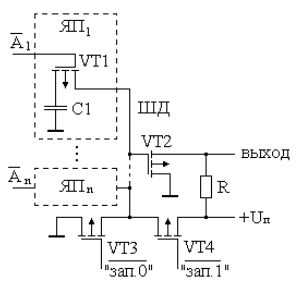
\includegraphics[scale=1]{a_dram_cell.png}  
  \caption{ Принципиальная схема ячейки ОЗУ динамического типа с элементами записи и усилителя считывания. }
  \label{fig:domain:ram:dram:dram_cell}
\end{figure}

Главное достоинство этой схемы - малая занимаемая площадь. Накопительный конденсатор C1 имеет МДП-структуру и изготавливается в едином технологическом цикле. Величина его емкости составляет сотые доли пикоФарад. Конденсатор C1 хранит информационный заряд. Транзистор VT1 выполняет роль переключателя, передающего заряд конденсатора в разрядную шину данных ШД при считывании, либо заряжающего конденсатор при записи. В режиме хранения на адресной линии A1 должен присутствовать потенциал логической единицы, под действием которого транзистор VT1 будет закрыт и конденсатор C1 отключен от шины данных ШД. Включение конденсатора в шину данных осуществляется логическим нулем на линии. При этом на транзистор VT1 подается напряжение, что приводит к его открыванию \cite{ibm_dram_article}.

Поскольку шина данных ШД объединяет все ячейки памяти данного столбца, то она характеризуется большой длиной и ее собственная емкость имеет существенное значение. Поэтому при открывании транзистора VT1 потенциал шины данных изменяется незначительно. Чтобы установившийся потенциал на ШД однозначно идентифицировать с уровнем напряжения логического нуля или логической единицы, используется усилитель на базе транзистора VT2 и резистора R. Непосредственно перед считыванием емкость шины данных подзаряжают подключением ее к источнику питания через транзистор VT4. Делается это для фиксации потенциала шины данных. При считывании информации происходит перераспределение заряда конденсатора и заряда шины данных, в результате чего информация, хранимая на конденсаторе С1, разрушается. Поэтому в цикле считывания необходимо произвести восстановление (регенерацию) заряда конденсатора. Для этих целей, а также для записи в ячейку памяти новых значений, используются транзисторы VT3 и VT4, которые подключают шину данных либо к источнику питания, либо к нулевому общему потенциалу. Для записи в ячейку памяти логической единицы необходимо открыть транзистор VT4 нулевым значением управляющего сигнала <</зап.1>> и подключить к шине данных источник питания. Для записи логического нуля необходимо нулевым потенциалом на входе «/зап.0» открыть транзистор VT3. Одновременная подача логических нулей на входы <</зап.1>>  и <</зап.0>> не допускается, так как это вызовет короткое замыкание источника питания на общий провод заземления.

На рисунке~\ref{fig:domain:ram:dram:dram_structure} показан пример структуры микросхемы динамического ОЗУ емкостью 64кбит. Данные в этой микросхеме памяти представлены как 64к отдельных бит, т.е. формат памяти 64к x 1. Ввод и вывод осуществляется раздельно, для чего предусмотрена пара выводов DI (вход) и DО (выход). Для ввода адреса имеется восемь контактов $A_0 - A_7$. Адресация к 64к ячейкам памяти осуществляется шестнадцатиразрядными адресами $A_0 - A_15$. Причем сначала на входы $A_0 - A_7$ подаются восемь младших разрядов $A_0 - A_7$ адреса, а затем – восемь старших разрядов $A_8 - A_15$. Восемь младших разрядов адреса фиксируются в регистре адреса строки подачей сигнала /RAS (сигнал выборки строки). Восемь старших разрядов адреса фиксируются в регистре адреса столбца подачей сигнала /CAS (сигнал выборки столбца). Такой режим передачи кода адреса называется мультиплексированным по времени. Мультиплексирование позволяет сократить количество выводов микросхемы. Ячейки памяти расположены в виде матрицы из 128 строк и 512 столбцов. Дешифратором строк вырабатывается адресный сигнал выборки $A_i$ ячеек памяти i-ой строки, т.е. выбирается одна из 128 строк. Обращение к строке вызывает подключение 512 ячеек памяти через соответствующие разрядные шины данных ШД этой строки к усилителям считывания (по одному на столбец). При этом автоматически происходит подзаряд запоминающих конденсаторов всех ячеек памяти выбранной строки до исходного уровня за счет передачи усиленного сигнала по цепи обратной связи. Этот процесс называется регенерацией памяти. Дешифратор столбцов выбирает один из 512 усилителей считывания. Бит, выбранный в режиме считывания, выдается на линию DО. Если одновременно с сигналом /CAS при предварительно установленном сигнале /RAS действует сигнал записи /WR, то бит с входа DI будет записан в выбранную ячейку памяти, при этом выход DО микросхемы остается в отключенном состоянии в течение всего цикла записи \cite{dram_tutorial}.

\begin{figure}[ht]
\centering
  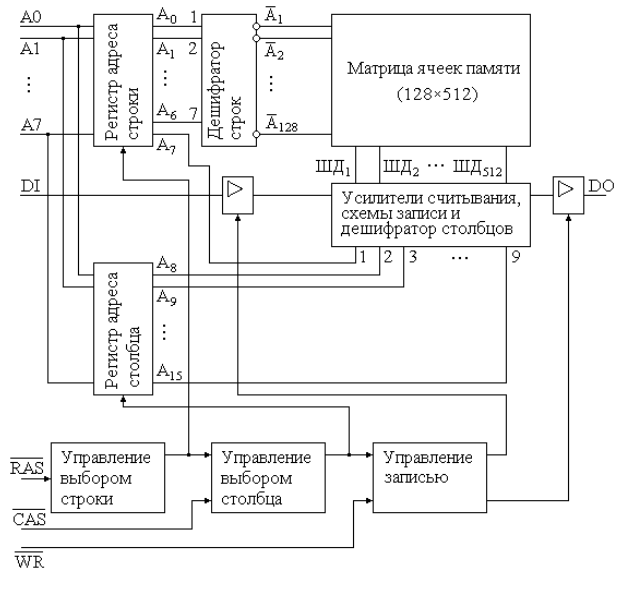
\includegraphics[scale=0.75]{a_dram_structure.png}  
  \caption{ Принципиальная схема ячейки ОЗУ динамического типа с элементами записи и усилителя считывания. }
  \label{fig:domain:ram:dram:dram_structure}
\end{figure}

На рисунке~\ref{fig:domain:ram:dram:dram_timing} представлены временные диаграммы, поясняющие работу динамического ОЗУ. В режиме считывания (рисунок~\ref{fig:domain:ram:dram:dram_timing},a) на адресные входы микросхемы подаются восемь младших разрядов $A_0 - A_7$ адреса, после чего вырабатывается сигнал /RAS, при этом производится выбор строки матрицы в соответствии с поступившим адресом. У всех ячеек памяти выбранной строки регенерируется заряд конденсаторов. Далее производится подача на адресные входы микросхемы восьми старших разрядов адреса, после чего вырабатывается сигнал /CAS. Этим сигналом выбирается нужная ячейка памяти из выбранной строки и считанный бит информации поступает на выход микросхемы DО. В режиме считывания промежуток времени между подачей сигнала /RAS и появлением данных на выходе DО называется временем выборки tв.

\begin{figure}[ht]
\centering
  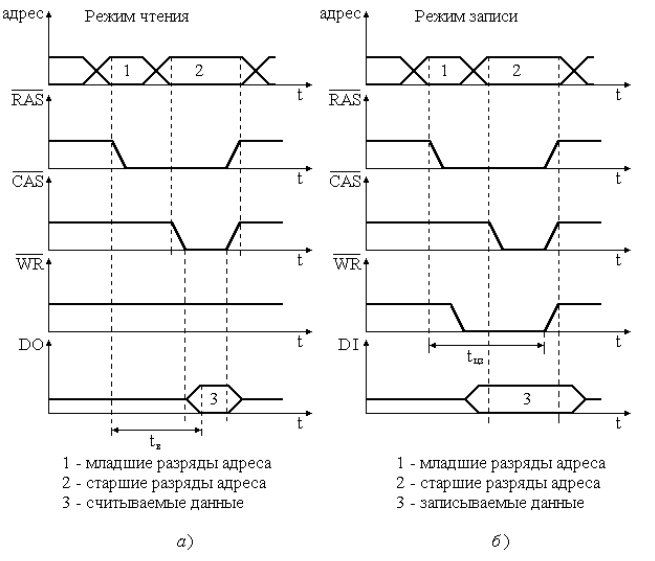
\includegraphics[scale=0.75]{a_dram_timing.png}  
  \caption{ Временная диаграмма работы ОЗУ динамического типа. }
  \label{fig:domain:ram:dram:dram_timing}
\end{figure}

В режиме записи (рисунок~\ref{fig:domain:ram:dram:dram_timing},б) за время цикла записи tцз принимается интервал времени между появлением сигнала /RAS и окончанием сигнала /WR. В момент появления сигнала /CAS записываемые данные уже должны поступать на вход DI. Сигнал /WR обычно вырабатывается раньше сигнала /CAS.

Для каждого типа микросхем динамических ОЗУ в справочниках приводятся временные параметры, регламентирующие длительность управляющих сигналов, подаваемых на микросхему, а также порядок их взаимного следования.
Заряд конденсатора динамического ОЗУ со временем уменьшается вследствие утечки, поэтому для сохранения содержимого памяти процесс регенерации каждой ячейки памяти должен производится через определенное время. Следовательно, для предотвращения разряда запоминающих конденсаторов необходимо обращаться к каждой строке матрицы через определенное время. При обычном режиме работы ОЗУ это условие не соблюдается, так как обращение к одним ячейкам происходит часто, а к другим очень редко. Поэтому необходим специальный блок, ответственный за регенерацию памяти. Этот блок должен при отсутствии обращений к ОЗУ со стороны внешних устройств циклически формировать на адресных входах $A_0 - A_6$ значения всех возможных адресов, сопровождая каждый из них управляющим сигналом /RAS, т.е. производить циклическое обращение ко всем 128 строкам матрицы ячеек памяти. Регенерацию необходимо проводить и в те моменты времени, когда ОЗУ используется устройствами, приостанавливая на время регенерации взаимодействие ОЗУ с этими устройствами, т.е. путем перевода этих устройств в режим ожидания.

Из изложенного выше следует, что использование динамического ОЗУ требует довольно сложной схемы управления. Если учесть, что обращение к ОЗУ со стороны устройств, с которыми оно работает, и обращение со стороны схемы регенерации не зависят друг от друга, следовательно, могут возникать одновременно, то необходима схема, обеспечивающая упорядоченность этих обращений. Для этих целей существуют схемы, управляющие работой динамических ОЗУ. Это так называемые контроллеры динамического ОЗУ, реализованные на одном кристалле. Их использование позволяет значительно упростить построение памяти на динамических ОЗУ.

Лидером в производстве микросхем динамического ОЗУ на сегодняшний день является фирма Samsung. Емкость одной микросхемы DRAM достигает значения 128 Мбайт и более. Кроме того, этой фирмой предлагается ряд передовых идей по обеспечению наибольшего быстродействия. Например, операции чтения и записи выполняются дважды за один такт – по переднему и заднему фронтам тактового импульса. Фирмой Mitsubishi предложена концепция встраивания в микросхемы динамической памяти статической кэш-памяти небольшого объема (Cashed DRAM), в которой хранятся наиболее часто запрашиваемые данные.

\subsection{Функциональные модели неисправностей ДОЗУ}
\label{sub:domain:faults}
Причиной неисправного состояния ОЗУ является наличие физического или механического дефекта либо множества подобных дефектов, количество и многообразие которых практически неограниченно. В зависимости от технологических особенностей при производстве ОЗУ и внешних факторов при его эксплуатации могут появляться новые типы и разновидности дефектов. Определение факта возникновения дефекта и его классификация представляется весьма трудоёмкой и зачастую неразрешимой задачей. 

Функциональные неисправности ОЗУ подразделяются на два подмножества: неисправности матрицы запоминающих элементов и неисправности электронного обрамления. Второе подмножество включает неисправности дешифратора адреса и неисправности логики чтения/записи. Доминирующее значение имеют неисправности матрицы запоминающих элементов ОЗУ.

К неисправностям матрицы запоминающих элементов ОЗУ относят неисправности, в которых участвуют: одна ячейка ОЗУ; две ячейки ОЗУ; несколько ячеек ОЗУ, в общем случае более чем две, без ограничений на их количество. 

К неисправностям, затрагивающим одну ячейку ОЗУ, относят \cite{faults}:

1. \textit{Константные неисправности} (Stuck-At Faults - SAF). Неисправный ЗЭ ОЗУ постоянно находится в состоянии логического нуля(SAF0) или логической единицы (SAF1), независимо от операций, выполняемых с неисправным ЗЭ и другими ЗЭ ОЗУ. Аналогично, как и для случая произвольной логики, различают однократные и многократные константные неисправности.

2. \textit{Переходные неисправности} (Transition Faults - TF). Подобные неисправности характеризуются невозможностью перехода состояния неисправного ЗЭ из 0 в 1 (TF1 $\uparrow$) или из 1 в 0 (TF $\downarrow$) при выполнении соответствующих операций записи. Данный тип неисправности достаточно близок по своей сути к константным неисправностям. Действительно, если ячейка, имеющая переходную неисправность, оказывается в состоянии, из которого она не может перейти в другое, ее поведение повторяет поведение ячейки, содержащей константную неисправность.

Среди неисправностей, в которых участвуют две ячейки ЗУ, выделяют следующие неисправности.

3. \textit{Неисправности взаимного влияния} (Coupling Fault - CF). При описании данной неисправности выделяют влияющий ЗЭ (i - Aggressor Cell), изменение логического состояния которого воздействует на состояние зависимого ЗЭ (j - Victim Cell). Различают три типа неисправностей взаимного влияния:
\begin{enumerate}
\item \textit{инверсные неисправности взаимного влияния} (Inverse Coupling Faults - CFin). При наличии данной неисправности изменение значения bi влияющего ЗЭ вызывает инвертирование значения $b_j$ зависимого ЗЭ. Возможны следующие виды неисправностей CFin: $\wedge$($\uparrow$, $b_j$*), $\wedge$($\downarrow$, $b_j$*), $\vee$($\uparrow$, $b_j$*), $\vee$($\downarrow$, $b_j$*). Символ $\wedge$ и символ $\vee$ задают взаимное расположение влияющего и зависимого запоминающих элементов ОЗУ. Первый символ $\wedge$ означает, что ЗЭ с меньшим адресом влияет на ЗЭ с большим адресом (i<j), а символ $\vee$ используется в случае, когда адрес влияющего ЗЭ больше адреса зависимого ЗЭ (i>j);
\item \textit{неисправности взаимного влияния прямого действия} (Idempotent Coupling Faults - CFid). При изменении значения bj влияющего ЗЭ происходит принудительная установка определённого логического значения 0 или 1 в зависимом ЗЭ. Различают восемь неисправностей прямого действия: $\wedge$($\uparrow$,0), $\wedge$($\uparrow$,1), $\wedge$($\downarrow$,0), $\wedge$($\downarrow$,1), $\vee$($\uparrow$,0), $\vee$($\uparrow$,1), $\vee$($\downarrow$,0) и $\vee$($\downarrow$,1). При исследовании эффективности тестов ОЗУ анализируется их покрывающая способность для всех 12 неисправностей взаимного влияния, в которых участвуют две ячейки (2-Coupling Faults) \cite{faults};
\item \textit{статические неисправности взаимного влияния} (State Coupling Faults -CFst). Переход зависимого ЗЭ в какое либо состояние $b_j$ возможен при определённом значении $b_i$ влияющего ЗЭ. Возможно восемь неисправностей CFst: $\wedge$(0,0), $\wedge$(0,1), $\wedge$(1,0), $\wedge$(1,1), $\vee$(0,0), $\vee$(0,1), $\vee$(1,0) и $\vee$(1,1).
\end{enumerate}

4. \textit{Кодочувствительные неисправности} (Pattern Sensitive Faults - PSF) рассматриваются как обобщение моделей неисправностей взаимного влияния. Для подобных неисправностей логическое состояние или изменение логического состояния одного ЗЭ ОЗУ может зависеть от содержимого (0 или 1) или от логических переходов из 1 в 0 или из 0 в 1 влияющих ЗЭ ОЗУ. В случае кодочувствительной неисправности PSF\textit{k}, в которой участвуют k запоминающих элементов ОЗУ, подразумевается, что влияющими ЗЭ в предельном случае могут быть любые \textit{k-1} из \textit{N} ЗЭ ОЗУ, а зависимым один из оставшихся \textit{N-k+1} ЗЭ. Такие неисправности называются неограниченными (Unrestricted) кодочувствительными неисправностями. Очевидно, что практическая значимость подобной модели невысока, так как сложность теста памяти и время его реализации при такой интерпретации кодочувствительной неисправности превышает всякие возможные пределы современных значений емкостей ЗУ. Поэтому при рассмотрении кодочувствительных неисправностей вводятся ограничения как на количество ЗЭ \textit{k}, так и на их местоположение \cite{faults}. 

При тестировании ОЗУ, как правило, придерживаются модели \textit{граничных кодочувствительных неисправностей} (Neighborhood Pattern Sensitive Faults - NPSF) как более реальной модели кодочувствительных неисправностей. Для таких моделей первым и необходимым ограничением является количество ЗЭ, участвующих в неисправности. Как правило, k не превышает 10, это следует из того факта, что для тестирования подобных неисправностей необходимо время пропорциональное величине $2^k$.
Вторым ограничением является физическое соседство ЗЭ. При этом зависимый ЗЭ называется \textit{базовым} ЗЭ (Base Cell), или базовой ячейкой, которая в данном случае является аналогом \textit{жертвы}, а остальные \textit{k-1} ЗЭ соседними ЗЭ (Neighborhood Cells), или \textit{соседними} ячейками, выступающими в роли агрессоров, количество и местоположение которых может быть произвольным. Поэтому на практике обычно используют модели кодочувствительных неисправностей NPSF\textit{k} с числом \textit{k}, равным 3, 5 и 9, конфигурации и обозначение которых приведены на рисунке~\ref{fig:domain:faults:neighbors}. 

\begin{figure}[ht]
\centering
  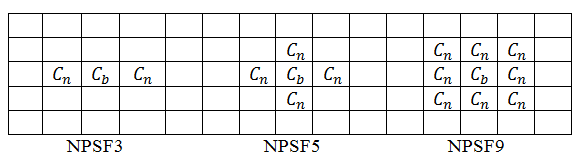
\includegraphics[scale=1]{a_faults_neighbors.png}  
  \caption{ Модели кодочувствительных неисправностей. }
  \label{fig:domain:faults:neighbors}
\end{figure}

Как видно из рисунка, в каждой из приведённых неисправностей в явном виде выделяется базовый ЗЭ - $C_b$ и соседние запоминающие элементы $C_n$, которые являются физическими соседями по отношению к базовому элементу.

В зависимости от эффекта влияния на базовый ЗЭ различают несколько классических типов кодочувствительных неисправностей NPSF\textit{k}.
\textit{Пассивными кодочувствительными неисправностями} (Passive NPSF - PNPSF) являются неисправности, при которых состояние базового ЗЭ не может быть изменено для определённого кода в \textit{k-1} соседних ЗЭ ОЗУ. 
\textit{Под активными кодочувствительными неисправностями} (Active NPSF - ANPSF) понимают неисправности, в которых базовый ЗЭ изменяет свое состояние из-за изменения кода в соседних ЗЭ. Изменение кода для подобных неисправностей происходит в результате изменения состояния на противоположное только в одном соседнем элементе, в то время как остальные ячейки сохраняют предыдущее состояние.
\textit{Статические кодочувствительные неисправности} (Static NPSF - SNPSF) характеризуются тем, что для определённой комбинации значений в соседних ЗЭ состояние базового ЗЭ принудительно устанавливается в состояние 0 или состояние 1. Главным отличием статических неисправностей от активных кодочувствительных неисправностей является длительность процесса установления неверного значения в базовой ячейке. Для статических неисправностей время существенно больше \cite{faults}.

Рассмотренные неисправности являются классическими и наиболее часто используются при тестировании ОЗУ. Однако существует и ряд других моделей неисправностей, также обсуждаемых и применяемых при тестировании памяти. В первую очередь здесь необходимо отметить \textit{неисправности дешифратора адреса} (Address Decoder Faults - AF), или \textit{адресные неисправности}. Однако обнаружение подобных неисправностей обеспечивается тестами, обнаруживающими неисправности матрицы ЗЭ.

Также к электронному обрамлению в большей мере относятся \textit{неисправности типа обрыв} (Stuck Open Fualt - SOF), которые также могут быть обнаружены при тестировании матрицы ОЗУ.
Логика чтение/запись обеспечивает интерфейс между массивом ячеек и внешней шиной данных. Данный функциональный блок может содержать те же типы неисправностей, что и массив ячеек памяти (SAF, TF, CFin, CFid). 
Модель типа \textit{разрушающая операция чтения} (Read Disturb Fault Model - RDF) практически аналогична неисправности \textit{слабый запоминающий элемент} (Weak Cell Fault Model - WCF) и обнаруживается путем внесения в классический маршевый тест временной задержки перед выполнением следующего маршевого элемента. Для ДОЗУ также характерна \textit{неисправность сохранения данных} (Data Retention Fault - DRF), которая, так же, как и неисправность RDF И WCF, обнаруживается путем внесения временных задержек в тест памяти.  

\subsection{Алгоритмы тестирования ДОЗУ}
\label{sub:domain:tests}
В условиях постоянного усложнения разрабатываемых средств электронной техники, как функционального, так и структурного (уже сегодня на подложке микропроцессора может быть расположено несколько миллионов транзисторов), в условиях необходимости быстрого продвижения уже разработанных устройств на рынок (быстрое моральное устаревание средств вычислительной техники) проблема надежного тестирования современных микропроцессоров и микропроцессорных систем становится все более актуальной. При этом очевидно, что качество и оперативность проектирования, эффективность и надежность функционирования микропроцессоров и микропроцессорных систем существенно зависят от качества и достоверности результатов решения задач их тестового диагностирования.

Рассмотрим классические методы тестирования ОЗУ.

\subsubsection{Тестирующий алгоритм Zero-One}
\label{sub:domain:tests:zero-one}
Тест Zero-One также известен как MSCAN. Он является достаточно простым и состоит из следующих шагов:
\begin{enumerate}
\item Запись 0 во все ячейки памяти;
\item Чтение ячеек памяти с ожидаемым значением 0;
\item Запись 1 во все ячейки памяти;
\item Чтение ячеек памяти с ожидаемым значением 1.
\end{enumerate}
Сложность данного теста составляет 4n. Не все неисправности типа Afs обнаруживаются. Неисправности типа SAFs обнаруживаются при условии исправного дешифратора адресов. Не все TFs и CFs обнаруживаются.

\subsubsection{Тестирующий алгоритм Checkboard}
\label{sub:domain:tests:checkboard}
Данный алгоритм предполагает создание сетки из нулей и единиц в шахматном порядке, как представлено на рисунке~\ref{fig:domain:tests:checkboard}. 

\begin{figure}[ht]
\centering
  
\includegraphics[scale=0.5]{a_test_checkboard.jpg}  
  \caption{ Состояние ячеек памяти при тестировании алгоритмом Checkboard. }
  \label{fig:domain:tests:checkboard}
\end{figure}

Алгоритм теста состоит из следующих шагов:
\begin{enumerate}
\item Запись 0 во все черные ячейки памяти и 1 во все белые ячейки;
\item Чтение всех ячеек памяти;
\item Запись 1 во все черные ячейки памяти и 0 во все белые ячейки;
\item Чтение всех ячеек памяти.
\end{enumerate}

Сложность теста составляет 4n. Тест обнаруживает не все неисправности Afs. SAFs обнаруживаются при условии исправного дешифратора адресов. Не все TFs и CFs обнаруживаются. В данном алгоритме важно построить шахматную доску на физической сетке элементов, а не на логическом уровне.

\subsubsection{Тестирующий алгоритм GALPAT}
\label{sub:domain:tests:galpat}
Алгоритм GALPAT (Galloping Pattern) состоит в заполнении памяти 0 (1), кроме базовой ячейки (base-cell), которая содержит 1 (0). На протяжении теста базовая ячейка перемещается по всей матрице. Тест проиллюстрирован на рисунке~\ref{fig:domain:tests:galpat}.

\begin{figure}[ht]
\centering
  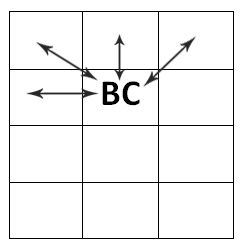
\includegraphics[scale=0.75]{a_test_galpat.png}  
  \caption{ Тестирующий алгоритм GALPAT. }
  \label{fig:domain:tests:galpat}
\end{figure}

Сложность алгоритма составляет $ 4n^{2} $. Покрывающая способность теста достаточно высокая, все неисправности типа Afs, TFs, CFs и SAFs обнаруживаются и локализуются. Псевдокод теста приведён в листинге~\ref{lst:domain:tests:galpat}.

\begin{lstlisting}[style=fsharpstyle, mathescape,escapeinside={/*@}{@*/},caption={Псевдокод реализации алгоритма GALPAT}, label=lst:domain:tests:galpat]
function GALPAT =
 Write background 0;
 for i in 0 .. 1 do
  for BC in 0 .. N-1 do
   Complement BC;
   for OC in 0 .. N-1 and OC != BC do
    Read BC;
    Read OC
   end for
   Complement BC;
   Write background 1;
 end for
end
\end{lstlisting}

\subsubsection{Тестирующий алгоритм WALPAT}
\label{sub:domain:tests:walpat}
Алгоритм WALPAT (Walking Pattern) очень похож на тест GALPAT. Различие лишь в том, что базовая ячейка считывается после того, как все остальные ячейки были просканированы. Сложность составляет $ 2n^{2} $. Тест проиллюстрирован на рисунке~\ref{fig:domain:tests:walpat}.

\begin{figure}[ht]
\centering
  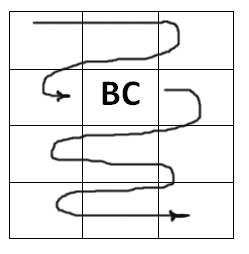
\includegraphics[scale=0.75]{a_test_walpat.png}  
  \caption{ Тестирующий алгоритм WALPAT. }
  \label{fig:domain:tests:walpat}
\end{figure}

Покрывающая способность данного теста, как и алгоритма Galloping Pattern, достаточно высокая, все неисправности типа Afs, TFs, CFs и SAFs обнаруживаются и локализуются. Псевдокод теста приведён в листинге~\ref{lst:domain:tests:walpat}.

\begin{lstlisting}[style=fsharpstyle, mathescape,escapeinside={/*@}{@*/},caption={Псевдокод реализации алгоритма WALPAT}, label=lst:domain:tests:walpat]
function WALPAT =
 Write background 0;
 for i in 0 .. 1 do
  for BC in 0 .. N-1 do
   Complement BC;
   for OC in 0 .. N-1 and OC != BC do
    Read OC
   end for
   Read BC;
   Complement BC;
   Write background 1;
 end for
end
\end{lstlisting}

\subsubsection{Тестирующий алгоритм Sliding}
\label{sub:domain:tests:sliding}
Тест основывается на алгоритме GALPAT, но вместо сдвига 1 по матрице ячеек, сдвигается целая диагональ(колонка, ряд) единиц. После каждого сдвига сканируется вся память. Визуально тест представлен на рисунке~\ref{fig:domain:tests:sliding}.

\begin{figure}[ht]
\centering
  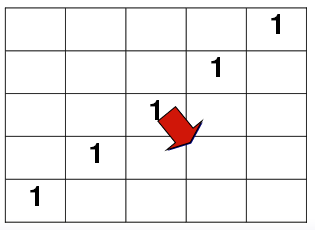
\includegraphics[scale=0.75]{a_test_sliding.png}  
  \caption{ Тестирующий алгоритм Sliding. }
  \label{fig:domain:tests:sliding}
\end{figure} 

Сложность алгоритма составляет $ 4n^{1.5} $. Покрывающая способность теста также довольно высокая, обнаруживаются все неисправности, за исключением некоторых неисправностей типа CFs.

\subsubsection{Тестирующий алгоритм Butterfly}
\label{sub:domain:tests:butterfly}
На протяжении теста базовая ячейка сдвигается по матрице памяти. При каждом сдвиге в цикле проверяются её ближайшие соседи в радиусе не более половины от длины строки и столбца матрицы ячеек. Тест представлен на рисунке~\ref{fig:domain:tests:butterfly}. 

\begin{figure}[ht]
\centering
  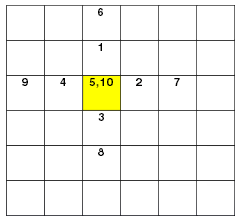
\includegraphics[scale=0.75]{a_test_butterfly.png}  
  \caption{ Тестирующий алгоритм Butterfly. }
  \label{fig:domain:tests:butterfly}
\end{figure} 

Сложность алгоритма составляет $ 5n \log n $. Тест обнаруживает все неисправности типа SAFs и некоторые из AFs. Псевдокод теста приведён в листинге~\ref{lst:domain:tests:butterfly}.

\begin{lstlisting}[style=fsharpstyle, mathescape,escapeinside={/*@}{@*/},caption={Псевдокод реализации алгоритма Butterfly}, label=lst:domain:tests:butterfly]
function Butterfly =
 Write background 0;
 For i in 0 .. 1 do
  For BC in 0 .. N-1 do
   Complement BC;
   dist = 1; 
   While dist <= mdist do// mdist < 0.5 col/row length
    Read cell dist north from BC;
    Read cell dist east from BC;
    Read cell dist south from BC;
    Read cell dist west from BC;
    Read BC; 
    dist *=2;
   end while
   Complement BC
  end for
  Write background 1
 end for
end
\end{lstlisting}

\subsubsection{Тестирующий алгоритм Surround Disturb}
\label{sub:domain:tests:sd}
Алгоритм SD (Surround Disturb) Позволяет проверить поведение ячеек в строке, когда комплиментарные значения записываются в ячейки, расположенные на соседних рядах матрицы. Этот алгоритм разработан на предположении, что ячейки памяти наиболее чувствительны к помехам от своих ближайших соседей. Тест представлен на рисунке~\ref{fig:domain:tests:sd}. 

\begin{figure}[ht]
\centering
  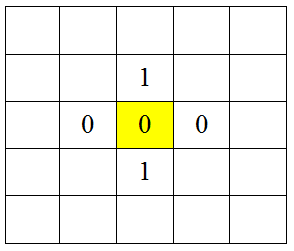
\includegraphics[scale=0.75]{a_test_sd.png}  
  \caption{ Тестирующий алгоритм Surround Disturb. }
  \label{fig:domain:tests:sd}
\end{figure} 

Псевдокод алгоритма представлен в листинге~\ref{lst:domain:tests:sd}.

\begin{lstlisting}[style=fsharpstyle, mathescape,escapeinside={/*@}{@*/},caption={Псевдокод реализации алгоритма Surround Disturb}, label=lst:domain:tests:sd]
For each cell [p,q] // row = p, col = q
{
 write 0 in cell[p,q-1];
 write 0 in cell[p,q];
 write 0 in cell [p, q+1];
 write 1 in cell[p-1,q];
 read 0 from cell[p,q+1];
 write 1 in cell[p+1,q];
 read 0 from cell[p, q-1];
 read 0 from cell[p,q];
}
\end{lstlisting}

\subsubsection{Маршевые тесты}
\label{sub:domain:tests:march}
Маршевые тесты являются самыми простыми и оптимальными для тестирования памяти. Они имеют линейную сложность и симметрию.
Маршевый тест состоит из конечной последовательности маршевых элементов. В свою очередь маршевый элемент состоит из последовательности операций чтения и записи, которые применяются ко всем ячейкам памяти в возрастающем или убывающем порядке адресов.
Все операции маршевого элемента выполняются до перехода к следующей ячейке памяти.
Обозначается маршевый элемент следующим образом: $rx$ - чтение из ячейки памяти, в которой должно храниться значение $x$; $wx$ - запись в ячейку памяти значения $x$; $\Uparrow$ - возрастающий порядок адресов (от 0 до n-1); $\Downarrow$ - убывающий порядок адресов (от n-1 до 0); $\Updownarrow$ - возрастающий или убывающий порядок адресов (направление не важно). 

Пример маршевого теста: $\{\Uparrow (w1); \Uparrow (r1,w0)\}$. Такой маршевый тест предполагает следующий алгоритм:

\begin{enumerate}
\item Проходя от 0 до n-1 ячейки памяти записать 1 в i-ую ячейку;
\item Проходя от 0 до n-1 ячейки памяти прочитать значение из i-ой ячейки, в которой должна быть 1, и записать в эту ячейку 0;
\end{enumerate}

В таблице~\ref{table:domain:tests:march_tests} представлены некоторые маршевые тесты.

\begin{table}[ht]
  \caption{Маршевые тесты}
  \label{table:domain:tests:march_tests}
  \begin{tabular}{| >{\centering}m{0.2\textwidth}
                  | >{\centering\arraybackslash}m{0.7\textwidth}|}
   \hline 
  {Наименование} & {Алгоритм} \\ \hline
   MATS & $\{\Updownarrow (w0); \Updownarrow (r0,w1); \Updownarrow (r1)\}$ \\ \hline
   MATS+ & $\{\Updownarrow (w0); \Uparrow (r0,w1); \Downarrow (r1,w0)\}$ \\ \hline
   MATS++ & $\{\Updownarrow (w0); \Uparrow (r0,w1); \Downarrow (r1,w0,r0)\}$ \\ \hline
   March X & $\{\Updownarrow (w0); \Uparrow (r0,w1); \Downarrow (r1,w0); \Updownarrow (r0)\}$ \\ \hline
   March C- & $\{\Updownarrow (w0); \Uparrow (r0,w1); \Uparrow (r1,w0); \Downarrow (r0,w1); \Downarrow (r1,w0); \Updownarrow (r0)\}$ \\ \hline
   March A & $\{\Updownarrow (w0); \Uparrow(r0,w1,w0,w1); \Uparrow (r1,w0,w1); \Downarrow (r1,w0,w1,w0); \Downarrow (r0,w1,w0)\}$ \\ \hline
   March B & $\{\Updownarrow (w0); \Uparrow(r0,w1,r1,w0,r0,w1); \Uparrow (r1,w0,w1); \Downarrow (r1,w0,w1,w0); \Downarrow (r0,w1,w0)\}$ \\ \hline
  \end{tabular}
\end{table}

Важным этапом в эволюции функциональных тестов ОЗУ стало применение неразрушающих методов тестирования. Необходимость в их использовании обусловлена критичностью современных приложений (сетевые серверы, системы управления) к показателям надежности\cite{March_Tests_Ivaniuk}. В таких случаях необходимо использовать тестовые алгоритмы, которые не разрушали бы содержимое ОЗУ. Преобразовать разрушающий маршевый тест в его неразрушающий аналог достаточно просто. Неразрушающие тесты имеют ряд обязательных требований: любой маршевый элемент начинается операцией чтения, отсутствует начальная инициализация памяти ($\Updownarrow (wx)$). После выполнения теста необходимо вернуть память в её первоначальное состояние. Идея неразрушающих тестов состоит в замене операций чтения и записи конкретных значений на операции чтения и записи прямых и обратных (комплиментарных) значений, хранящихся в ячейках памяти. 
Теперь неразрушающие операции маршевых тестов примут следующий вид: wdc, wd - запись dc и d значений в ячейку памяти; rdc, rd - чтение из ячейки памяти ожидаемых значений dc и d. Значение dc есть комплиментарное значение к d. На примере теста MATS+ его неразрушающий аналог будет выглядеть следующим образом: $\{\Uparrow (rd,wdc); \Downarrow (rdc,wd)\}$.

\subsection{Обзор существующих аналогов}
\label{sub:domain:analogue}
В открытых источниках информация о существующих аналогах не найдена. Даже если таковые имеются, то они скорее всего являются закрытыми инструментами компаний, занимающихся проблемой тестирования памяти. Вследствие этого факта сравнение с ними невозможно. Исходя из отсутствия свободно распространяемых утилит по верификации тестирующих алгоритмов ОЗУ, разработка данного программного средства имеет смысл.

\subsection{Постановка задачи}
\label{sub:domain:task}
В результате выполнения дипломного проекта должна быть разработана библиотека, написанная на языке С++, для верификации тестирующих алгоритмов оперативных запоминающих устройств со следующими спецификациями:
\begin{itemize}
  \item Разрабатываемое ПО должно иметь возможность запускаться под платформами Windows(7,8,10);
  \item Разрабатываемое ПО должно позволять производить верификацию тестирующих алгоритмов ОЗУ, в зависимости от требований
конечного пользователя;
  \item Подвергаться тестированию должна динамическая память, симулируемая инструментом DRAMSim2
  \item Время работы ПО должно быть приемлемым.
\end{itemize}






\lstset{style=fsharpstyle}

\section{Используемые технологии}
\label{sec:practice:technology_used}

Выбор технологий является важным предварительным этапом разработки сложных информационных систем.
Платформа и язык программирования, на котором будет реализована система, заслуживает большого внимания, так как исследования показали, что выбор языка программирования влияет на производительность труда программистов и качество создаваемого ими кода.

Ниже перечислены некоторые факторы, повлиявшие на выбор технологий:
\begin{itemize}
\item Разрабатываемое ПО должно иметь возможность запускаться под платформами Windows(7,8,10) и Linux(Ubuntu, arch linux, freebsd)
\item Дальнейшей поддержкой проекта, возможно, будут заниматься разработчики, не принимавшие участие в выпуске первой версии.
\item Имеющийся разработчик имеет опыт работы с объекто"=ориентированными языками программирования.
\end{itemize}

Основываясь на опыте работы имеющихся программистов разрабатывать ПО целесообразно с помощью языка С++.
Приняв во внимание необходимость обеспечения доступности дальнейшей поддержки ПО, возможно, другой командой программистов, необходимость работы с различными ОС, целесообразно не использовать малоизвестные и сложные языки программирования.
Так как при разработке програмного средства будет использоваться симулятор DRAM, написанный на С++, целесообразно выбрать именно этот язык для создания внешней среды для этого симулятора.
Таким образом, с учетом вышеперечисленных факторов, целесообразно остановить выбор на следующих технологиях:
\begin{itemize}
  \item операционные системы: семейство Windows(7,8,10), семейство Linux\\(Ubuntu, Debian, Arch Linux);
  \item язык программирования С++.
\end{itemize}
Для реализации поставленной задачи предпочительно использовать стандартную библиотеку STL без использования сторонних библиотек для обеспечения простой компиляции проекта под любой операционной системой.
Высокий уровень абстракции языка, полноценные механизмы ООП, большое количество контейнеров и алгоритмов библиотеки STL позволяют наиболее просто и <<красиво>> решить поставленную задачу.
Разрабатываемое программное обеспечение в некоторой степени использует данное преимущество языка.

Далее проводится характеристика используемых технологий и языка программирования более подробно.

\subsection{Язык программирования С++}
\label{sub:practice:cpp_overview}
С++ - компилируемый, статически типизированный язык программирования общего назначения. Синтаксис C++ унаследован от языка C. Одним из принципов разработки было сохранение совместимости с C. Тем не менее, C++ не является в строгом смысле надмножеством C; множество программ, которые могут одинаково успешно транслироваться как компиляторами C, так и компиляторами C++, довольно велико, но не включает все возможные программы на C.

Язык поддерживает такие парадигмы программирования, как процедурное программирование, объектно-ориентированное программирование, обобщённое программирование, обеспечивает модульность, раздельную компиляцию, обработку исключений, абстракцию данных, объявление типов (классов) объектов, виртуальные функции. Стандартная библиотека включает, в том числе, общеупотребительные контейнеры и алгоритмы. C++ сочетает свойства как высокоуровневых, так и низкоуровневых языков. В сравнении с его предшественником — языком C, — наибольшее внимание уделено поддержке объектно-ориентированного и обобщённого программирования \cite{cpp_book}.

C++ широко используется для разработки программного обеспечения, являясь одним из самых популярных языков программирования. Область его применения включает создание операционных систем, разнообразных прикладных программ, драйверов устройств, приложений для встраиваемых систем, высокопроизводительных серверов, а также развлекательных приложений (игр). Существует множество реализаций языка C++, как бесплатных, так и коммерческих и для различных платформ. Например, на платформе x86 это GCC, Visual C++, Intel C++ Compiler, Embarcadero (Borland) C++ Builder и другие. C++ оказал огромное влияние на другие языки программирования, в первую очередь на Java и \csharp{}.

Главное нововведение C++ - механизм классов, дающий возможность определять и использовать новые типы данных. Программист описывает внутреннее представление объекта класса и набор функций-методов для доступа к этому представлению. Одной из заветных целей при создании C++ было стремление увеличить процент повторного использования уже написанного кода. Концепция классов предлагала для этого механизм наследования. Наследование позволяет создавать новые (производные) классы с расширенным представлением и модифицированными методами, не затрагивая при этом скомпилированный код исходных (базовых) классов. Вместе с тем наследование обеспечивает один из механизмов реализации полиморфизма - базовой концепции объектно-ориентированного программирования, согласно которой, для выполнения однотипной обработки разных типов данных может использоваться один и тот же код. Собственно, полиморфизм - тоже один из методов обеспечения повторного использования кода \cite{cpp_book_two}.

Введение классов не исчерпывает всех новаций языка C++. В нем реализованы полноценный механизм структурной обработки исключений, отсутствие которого в С значительно затрудняло написание надежных программ, механизм шаблонов - изощренный механизм макрогенерации, глубоко встроенный в язык, открывающий еще один путь к повторной используемости кода, и многое другое.

Таким образом, генеральная линия развития языка была направлена на расширение его возможностей путем введения новых высокоуровневых конструкций при сохранении сколь возможно полной совместимости с ANSI С. Конечно, борьба за повышение уровня языка шла и на втором фронте - те же классы позволяют при грамотном подходе упрятывать низкоуровневые операции, так что программист фактически перестает непосредственно работать с памятью и системно-зависимыми сущностями.

\subsection{Симуляторы ДОЗУ}
\label{page:domain:simulators}

Для моделирования процессов оперативной памяти используется множество симуляторов, от упрощенных моделей, которые лишь регулируют временные задержки и пропускную способность доступа к памяти, и до детализированных симуляторов, которые могут точно отразить сложное поведение современных систем памяти. К сожалению, в открытом доступе находится малая их часть. В этом разделе будут рассмотрены и сравнены некоторые симуляторы, информация о которых имеется в открытых источниках.

\subsubsection{DRAMSim2}~\\
\label{page:domain:simulators:dramsim2}

Одним из популярных симуляторов памяти является DRAMSim2, разработанный в университете Мэриленд, США. 
DRAMSim2 – это потактовый симулятор оперативной памяти, реализованный на языке С++ как объектно-ориентированная модель DDR2/3 памяти. Помимо прочего данный симулятор обеспечивает надежный инструмент для визуализации и сравнения влияния системных параметров памяти на ключевые метрики производительности, такие как пропускная способность, временные задержки и потребляемую мощность \cite{dramsim2_article}.

Ядро симулятора заключено в единый объект, который называется MemorySystem. Он состоит из двух компонент: контроллера памяти и ОЗУ. Диаграмма главных компонентов симулятора DRAMSim2 и их связей изображена на рисунке~\ref{fig:domain:simulators:dramsim2:dramsim2_component}. 

\begin{figure}[ht]
\centering
  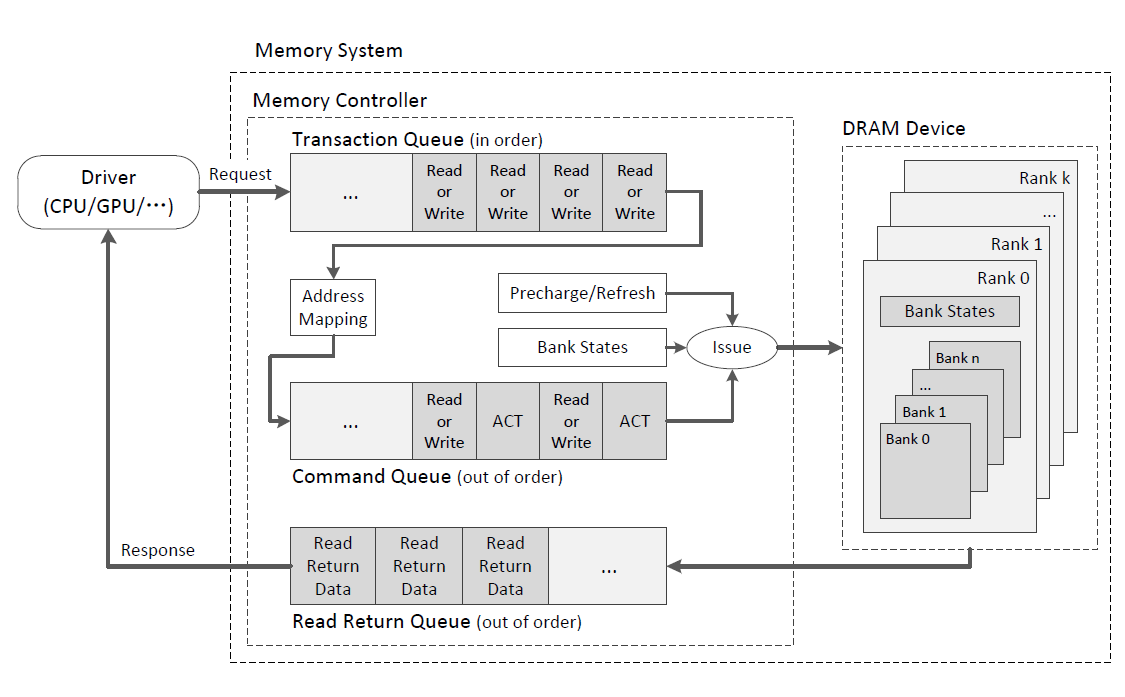
\includegraphics[scale=0.4]{a_dramsim2_components.png}  
  \caption{ Диаграмма компонентов симулятора DRAMSim2. }
  \label{fig:domain:simulators:dramsim2:dramsim2_component}
\end{figure}

Для объекта MemorySystem необходимо наличие двух ini-файлов: для инициализации системы в целом и для описания ОЗУ. Файл инициализации ОЗУ содержит описание параметров конкретного устройства, таких как временные ограничения и параметры энергопотребления устройства. Значения этих параметров можно найти в справочных данных, предоставляемых производителями ОЗУ.

Пакет DRAMSim2 содержит несколько ini-файлов для устройств Micron DDR2/3 различного объёма и скорости. Ini-файл системы содержит параметры, независящие от конкретного типа ОЗУ. Они включают в себя такие параметры, как схемы отображения адресов, опции отладки, структура очереди контроллера памяти и другие детали симуляции.

После создания объекта  MemorySystem код драйвера памяти должен зарегистрировать функции обратного вызова, чтобы получать уведомления о выполнении запросов. На этом этапе инициализация симулятора завершена. Код драйвера должен вызывать специальную функцию для каждого системного такта, а также другую функцию, для добавления запроса к памяти. По окончании обработки запроса симулятор информирует драйвер о выполненном действии, вызывая зарегистрированную функцию обратного вызова \cite{dramsim2_manual}.

Поскольку вся логика взаимодействия с симулятором заключена в простом интерфейсе с минимальным количеством функций, симулятор  легко внедрить в любую систему, будь то простой драйвер или потактовый симулятор ЦП, такой как MARSSx86. 
DRAMSim2 может быть скомпилирован как автономный исполняемый модуль, либо же в качестве библиотеки. Соответственно симулятор работает в двух режимах : автономном и встроенном в другую систему. В автономном режиме симулятор считывает список команд из trace-файла, хранящегося на диске. Во встроенном режиме симулятор предоставляет базовую функциональность для создания объекта системы памяти и добавления запросов к нему. 

DRAMSim2 не использует никаких сторонних библиотек, кроме стандартной библиотеки C++ STL. Благодаря этому симулятор легко скомпилировать под любой операционной системой, на которой установлен компилятор GNU C++. Для запуска симулятора под OС Windows потребуется Cygwin.

Поскольку производители отказываются публиковать детали работы их контроллеров памяти, DRAMSim2 моделирует современные DDR2/3 контроллеры в общем виде. Запросы от драйвера (любой модуль, который выдаёт запросы, например центральный процессор) накапливаются в очереди транзакций в порядке их выполнения.  Эти транзакции преобразуются в команды ОЗУ и направляются в очередь команд, а затем выдаются запоминающему устройству. Контроллер памяти отслеживает состояние каждого банка памяти, на основе чего определяет, какой запрос должен быть передан ОЗУ следующим. Взаимодействие драйвера, контроллера памяти и DRAM отображено на рисунке~\ref{fig:domain:simulators:dramsim2:dramsim2_component}. Выдача запросов в случайном порядке помогает оптимизировать использование банка и тем самым повысить пропускную способность памяти и уменьшить задержки.

После получения устройством DRAM команды и данных от контроллера памяти, список состояний банков используется для проверки ошибок, чтобы убедиться, что время полученной команды верное. 

В дополнение к моделированию изменения состояния системы во время операций чтения и записи, контроллер памяти DRAMSim2 так же моделирует эффект восстановления памяти ОЗУ. Моделирование регенерации памяти имеет важное значение, так как операции восстановления являются основным источником задержек при выполнении запросов к памяти. Запросы чтения, поступившие во время восстановления памяти, должны ожидать обработки намного дольше, чем другие запросы. 

Достоинством симулятора DRAMSim2 является простой интерфейс, общедоступный исходный код, который можно скачать с сайта GitHub.com, подробная документация, наличие готовых конфигурационных файлов для различных типов памяти. Симулятор легко скомпилировать под любой операционной системой, при этом не требуется инсталляция дополнительных библиотек.  В качестве серьёзного недостатка является отсутствие в бесплатной версии симулятора возможности записи и считывания данных, но относительная простота кода и грамотная архитектура системы позволяет программисту доработать этот момент.  

\subsubsection{Ramulator}~\\
\label{page:domain:simulators:ramulator}

Ramulator – это быстрый, потактовый DRAM симулятор, целью создания которого была потребность в расширяемом симуляторе, который может быль легко модифицирован под любой стандарт памяти, чтобы иметь представление о достоинствах современных DRAM \cite{ramulator_manual}.

В основе Ramulator лежит обобщённый шаблон для моделирования систем DRAM, который позже конкретизируется под определённый стандарт памяти. Благодаря такому гибкому дизайну симулятор может обеспечить поддержку широкого спектра стандартов DRAM: DDR3/4, LPDDR3/4, GDDR5, WIO1/2, HBM, а так же академических стандартов(SALP, AL-DRAM, TLDRAM, RowClone, and SARP).  Важно заметить, что данный симулятор не жертвует скоростью памяти для обеспечения такой расширяемости и гибкости. 

Ramulator основывается на важном наблюдении: любая DRAM может быть представлена в виде иерархии конечных автоматов, где поведение каждого автомата, как и иерархии в целом, диктуется стандартами DRAM.
Из любого предоставленного стандарта DRAM симулятор извлекает полную спецификацию для иерархии конечных автоматов и их поведения, которую затем объединяет в единый класс(например, DDR3.h/cpp). Вследствие этого симулятор легко переконфигурировать под другой стандарт памяти, что не требует изменений в коде.

На рисунке ~\ref{fig:domain:simulators:ramulator:code} представлен сласс DRAM, который является обобщенным шаблоном для построения иерархии(т.е. дерева) конечных автоматов (т.е. узлов). Экземпляр класса DRAM  - это один из узлов в дереве, который будет заключать в себе конкретную реализацию стандарта DRAM (DRAM<DDR3>).

\begin{figure}[ht]
\centering
  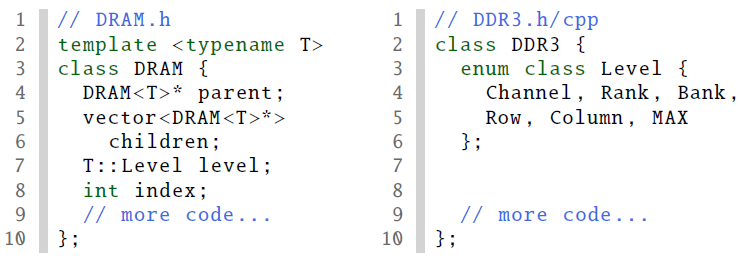
\includegraphics[scale=0.5]{a_ramulator_code.png}  
  \caption{ Обобщенный шаблон DRAM и его специализация. }
  \label{fig:domain:simulators:ramulator:code}
\end{figure}

На рисунке ~\ref{fig:domain:simulators:ramulator:tree} представлено полностью реализованное дерево, состоящее из узлов различного уровня: от канала до банка. Вместо того, чтобы создавать отдельный класс для каждого уровня (DDR3 Channel, DDR3 Rank, DDR3 Bank), Ramulator просто представляет каждый уровень как очередное свойство узла дерева. Это свойство может быть легко переназначено для адаптации иерархий под различные уровни. Ramulator так же предоставляет контроллер памяти, который взаимодействует с деревом через его корень. Каждый раз, когда контроллер памяти инициирует запрос или операцию, производится обход дерева, затрагивающий только необходимые узлы во время выполнения процесса.

\begin{figure}[ht]
\centering
  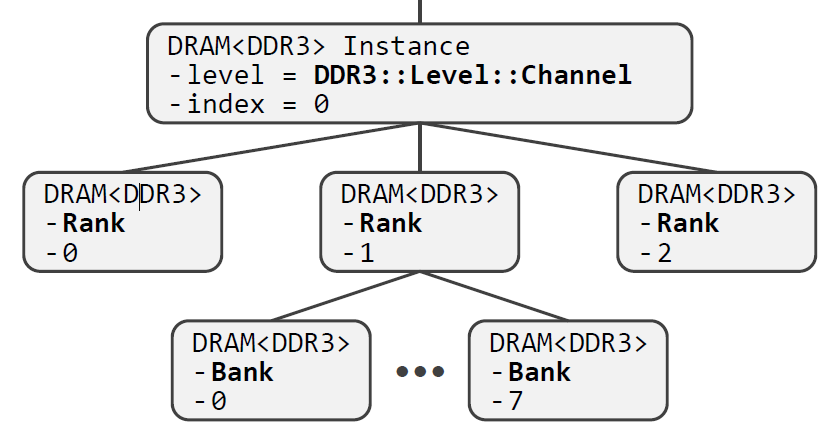
\includegraphics[scale=0.5]{a_ramulator_tree.png}  
  \caption{ дерево конечных автоматов памяти DDR3. }
  \label{fig:domain:simulators:ramulator:tree}
\end{figure}

Система конечных автоматов подразумевает набор состояний, переход между которыми осуществляется под внешним воздействием. Конечный автомат рассматриваемого симулятора хранит в себе текущее состояние, которое может принимать одно из значений, определяемых в классе конкретного вида памяти (например, DDR3). Узел может переходить из одного состояния в другое при получении одной из команд, которые так же определяются классом симулируемой памяти. Так же узел хранит в себе таблицу временных параметров, по которой определяется ближайшее время, через которое узел сможет принять ту или иную команду. Цель этой таблицы – предотвратить преждевременный переход узла из одного состояния в другое.  У каждого узла в дереве есть 3 функции: decode, check и update. Команда, поступившая к конкретному узлу, должна декодироваться. Функция decode распознаёт команду и проверяет возможность её выполнения, основываясь на статусе узла. Например, команда чтения не может быть выполнена, если rank отключен или bank закрыт. Для данной команды и адреса функция decode вернёт команду, которая должна быть выполнена перед командой чтения.  Даже если нет команд, которые должны быть предварительно выполнены перед операцией, это не означает, что поступившая команда может выполняться тут же. Например, bank может быть не готов к чтению, если он был активирован недавно. Для этих целей функция check сообщает, можно ли выполнить команду прямо сейчас (на текущем цикле). Если функция check разрешила выполнение команды, то контроллер памяти выполняет ее. Функция update в зависимости от команды модифицирует статус узла и его временные параметры в таблице.

Кроме того Ramulator поддерживает унифицированный контроллер памяти, который совместим со всеми стандартами DRAM(поддерживаемых в симуляторе). Контроллер памяти содержит три очереди запросов к памяти:  чтение, запись и техническое обслуживание. В то время, как очереди чтения/записи наполняются запросами, поступившими от внешнего источника команд (trace-файл с командами чтения и записи), очередь технического обслуживания узлов наполняется другим видом команд (обновление, отключение питания, автообновление), генерируемых внутри контроллера памяти, когда они необходимы. Для обработки запросов трёх очередей контроллер памяти взаимодействует с иерархическим деревом DRAM используя три функции узла, описанные выше.  

Таким образом Ramulator представляет собой расширяемый DRAM симулятор, обеспечивающий потактовую модель широкого разнообразия стандартов: DDR3/4, LPDDR3/4, GDDR5, WIO1/2, HBM, SALP, ALDRAM, TL-DRAM, RowClone, and SARP. Модульная архитектура системы позволяет легко дополнять симулятор новыми стандартами. Для некоторых стандартов Ramulator способен предоставлять отчеты по энергопотреблению. Ramulator оснащен простым контроллером памяти, представляющим из себя внешнее API для отправки и получения запросов памяти. Симулятор доступен в двух различных форматах : для автономного использования и для встроенного в систему режима. Для компиляции симулятора требуется компилятор GNU C++ и библиотека clang++. Из-за использования дополнительной библиотеки могут возникнуть трудности при компиляции проекта в операционной системе Windows. В бесплатной версии симулятора отсутствует возможность реального хранения данных.

\subsubsection{Обоснование выбора симулятора DRAM}~\\
\label{page:domain:simulators:simulator_choice}

Среди прочих симуляторов, информация о которых есть в открытом доступе, можно отметить еще несколько симуляторов. 

DrSim – потактовый симулятор DRAM памяти. Поддерживает стандарты памяти DDR2, DDR3 и LPDDR2. Написан на языке С++. Для компиляции потребуется GNU C++ и GNU Make. В целом этот симулятор очень напоминает DRAMSim2. Он так же работает в двух режимах: автономном и встроенном. В конфигурационных файлах задаются параметры для конкретного типа DRAM, а так же основные параметры для системы в целом. В режиме атвономной работы команды считываются из trace-файла, результаты выполнения выводятся на консоль. Во встроенном режиме внешней системе нужно выполнять роль генератора тактов для памяти, а так же отправлять запросы. По завершении выполнения запроса вызывается функция обратного вызова, чтобы позволить пользователю увидеть результаты выполнения команды \cite{drsim_manual}.

USIMM – симулятор DRAM, поддерживающий стандарт DDR3. Симулятор написан на языке С, без использования дополнительных библиотек. Главный модуль симулятора запускает цикл, в котором он получает команду из очереди запросов и запускает функцию updateMemory. Эту функцию реализует контроллер памяти, который проверяет временные параметры DRAM, чтобы определить, какие команды могут быть выполнены на данном цикле. Пользователь должен предоставить функцию scheduler, которая будет выдавать команды для каналов в каждый цикл работы памяти. В конфигурационных файлах описываются параметры для симулируемой памяти \cite{usimm_manual}.
 

Для сравнения симуляторов на рисунке~\ref{fig:domain:simulators:simulator_choice:comparison} приводятся параметры производительности каждого симулятора, запущенного на одном и том же trace-файле.

\begin{figure}[ht]
\centering
  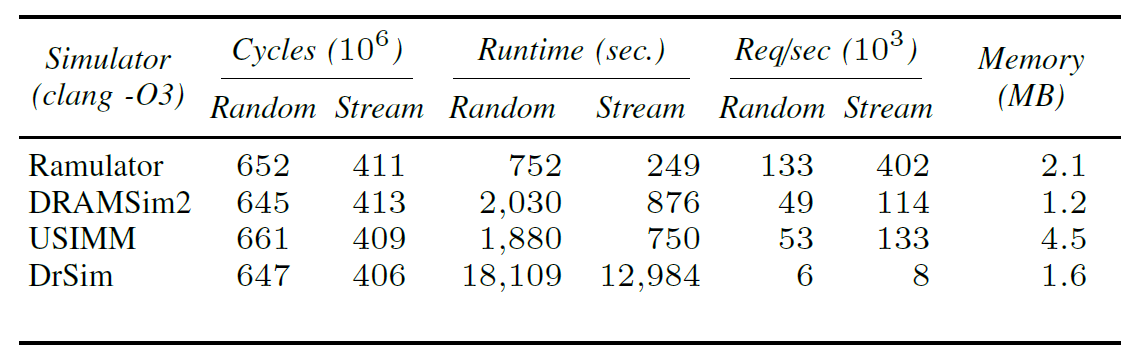
\includegraphics[scale=0.4]{a_simulators_comparison.png}  
  \caption{ Сравнение различных симуляторов DRAM. }
  \label{fig:domain:simulators:simulator_choice:comparison}
\end{figure}

Среди рассмотренных симуляторов Ramulator является наиболее гибкой и хорошо спроектированной моделью динамической памяти. Однако при попытке компиляции проекта под ОС Windows возникли проблемы с библиотекой clang++. Данный симулятор поддерживает широкий круг стандартов памяти, однако в рамках задачи дипломного проекта такой широты не требуется. Симулятор DRAMSim2 является относительно простым и небольшим проектом, который легко скомпилировать под любой операционной системой, при этом не требуется инсталляция дополнительных библиотек. Простой интерфейс позволяет легко встраивать симулятор в другие системы. Симуляторы DrSim и USIMM во многом уступают симулятору DRAMSim2. Как по наличию скромной документации, так и по грамотности построения структуры исходного кода и удобству использования. В открытом доступе отсутствуют симуляторы с возможностью хранения реальных данных, вследствие чего симулятор DRAMSim2 вполне подойдёт для дополнительных модификаций и адаптаций под текущую задачу проекта. 

%\section{Архитектура и модули системы} % (fold)
\label{sec:arch_and_mod}

\subsection{Основные компоненты симулятора}
\label{sub:arch_and_mod:modules}

Для симуляции динамической оперативной памяти был выбран симулятор DRAMSim2. Данный симулятор обладает рядом преимуществ: простота, независимость от сторонних библиотек, хорошо организованная внутренняя архитектура программы. 

Симулятор является потактовым, вследствие чего все основные классы унаследованы от единого базового класса SimulatorObject. В листинге~\ref{lst:arch_and_mod:modules:simulator_object} представлена его структура. Объект этого класса имеет единственное поле - счетчик currentClockCycle, который инкрементируется методом step. Таким образом все компоненты симулятора работают в единой временной плоскости. Метод update каждый производный класс имплементирует по-своему, вкладывая нужную ему функциональность.  

\begin{lstlisting}[style=cplusplusstyle, caption={Класс SimulatorObject}, label=lst:arch_and_mod:modules:simulator_object]
class SimulatorObject
{
public:
  uint64_t currentClockCycle;

  void step();
  virtual void update()=0;
};
\end{lstlisting}

Самыми важными компонентами симулятора являются три класса: MemorySystem, MemoryController и DRAMDevice. 
Класс MemorySystem является ядром симулятора, включающим в себя всю его функциональность. Класс имеет простой интерфейс, через который внешний драйвер взаимодействует с памятью. С помощью метода AddTransaction драйвер добавляет запрос в память. Метод Update нужно вызывать в конце каждого цикла. Отсчет циклов производит драйвер памяти. 

Класс MemoryController  накапливает запросы от драйвера в очереди транзакций, транслируя их затем в команды для устройства памяти.  
Сама память представлена классом DRAMDevice, включающим в себя классы Rank и Bank. В зависимости от конфигурации каждый Rank содержит в себе определенное количество объектов Bank. В классе Bank матрица ячеек памяти представлена картой, где номер ряда является ключом, а значение представляет собой вектор слов, чьи порядковые номера соответствуют колонкам ячеек. Класс Bank представлен в листинге~\ref{lst:arch_and_mod:modules:bank}.

\begin{lstlisting}[style=cplusplusstyle, caption={Класс Bank}, label=lst:arch_and_mod:modules:bank]
class Bank
    {
    public:
        Bank();
        ~Bank();

        void read(BusPacket *busPacket);
        void write(const BusPacket *busPacket);

    public:
        BankState currentState;

    private:
        typedef map<uint64_t, std::auto_ptr<std::vector<uint16_t>> > row_map;
        row_map rowEntries;
    };
\end{lstlisting}

Для данного симулятора в открытом доступе имеется версия с возможностью хранения данных, что значительно ускорило разработку программного средства. Симулируемая память является слово-ориентированной. По этой причине появилась необходимость добавления функциональности для записи конкретных бит, а не только слов, в ячейки памяти. В листинге~\ref{lst:arch_and_mod:modules:write_bit}. представлен метод writeBit, который записывает 0 или 1 (в зависимости от параметра set) в позицию bit в ячейке по адресу заданного ряда и колонки.

\begin{lstlisting}[style=cplusplusstyle, caption={Метод записи конкретных бит в слове}, label=lst:arch_and_mod:modules:write_bit]
void Bank::writeBit(int row, int col, int bit, bool set)
{
    auto row_ = rowEntries[row].get();

    if (set)
        (*row_)[col] |= 1 << bit;
    else
    {
        if ((*row_)[col] & (1 << bit))
            (*row_)[col] ^= 1 << bit;
    }
}
\end{lstlisting}

В целом работа всей системы представляет собой следующее: контроллер памяти накапливает в очереди транзакций запросы от драйвера; на каждом новом цикле работы системы контроллер памяти извлекает одну транзакцию из очереди, транслирует её адрес в значения номера ранка, банка, ряда и колонки ячейки памяти, преобразует пакет транзакции в команду для устройства памяти и помещает этот пакет в очередь команд; из очереди команд по одному пакету в цикл извлекается команда и контроллер памяти определяет, какое действие нужно совершить устройству памяти. Решение  зависит от множества факторов: состояния банков (например, команда чтения не может быть выполнена, если адресуемая ячейка не активна, в этом случае нужна предварительная команда Activate); контроллер регенерации, который может приостановить все транзакции в системе и запустить процесс обновления памяти. Каждую команду записи в память отслеживает адаптивный сигнатурный анализатор, о котором будет рассказано в следующих подразделах. Контроллер регенерации с помощью сигнатурного анализатора выясняет, были ли неполадки в памяти за время её работы, и при необходимости запускает тесты. Внутри самого ОЗУ находится контроллер неисправностей, который имитирует поведение ячеек с физическими неисправностями, а также контролирует процесс разрядки ячеек при длительном отсутствии команды Refresh. ОЗУ в свою очередь в ответ на команды чтения возвращает контроллеру памяти считанные данные, которые сохраняются в очереди пакетов чтения и затем отправляются драйверу. Основные модули системы представлены на рисунке~\ref{fig:arch_and_mod:modules:main_modules}.

\begin{figure}[ht]
\centering
  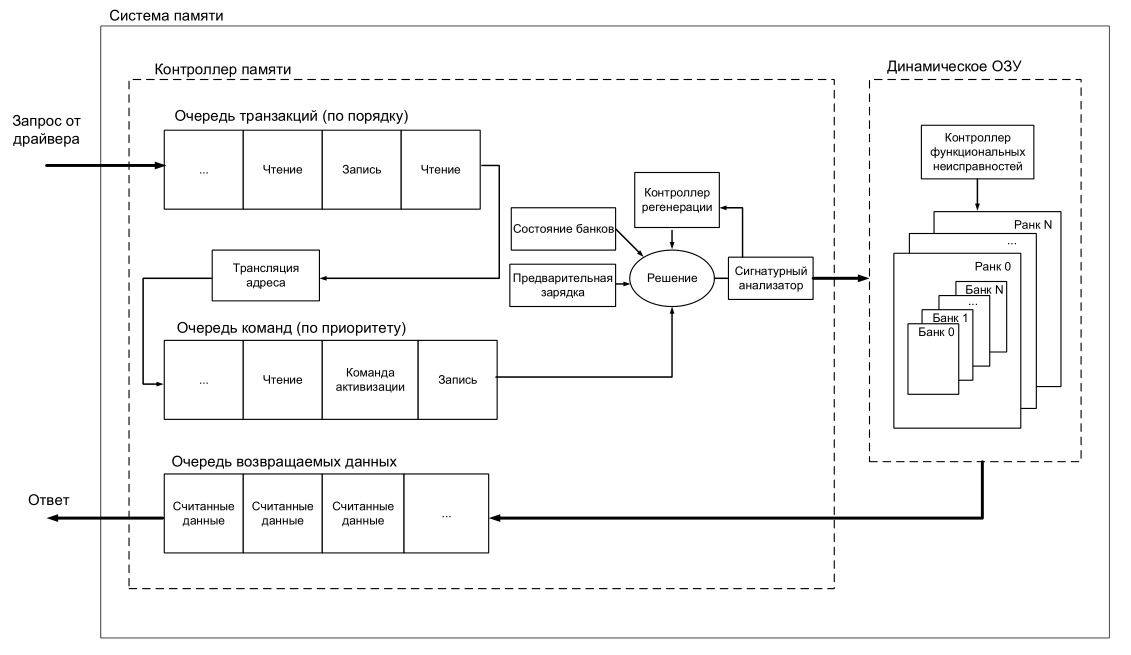
\includegraphics[scale=0.55]{a_main_modules.png}  
  \caption{ Основные компоненты симулятора ОЗУ. }
  \label{fig:arch_and_mod:modules:main_modules}
\end{figure}

\subsection{Симуляция процесса деградации памяти}
\label{sub:arch_and_mod:memory_discharge}

Источником ошибок может является свойство конденсаторов памяти разряжаться. Это происходит в случаях, когда период обновления памяти сдвинут и ячейки успевают терять свой заряд.

Этот процесс симулирует класс Discharger, который следит за периодами обновления памяти, и если такой период не наступил вовремя, то начинается постепенная деградация отдельных бит памяти в случайных местах (биты теряют свои данные и хранят 0). 

Для генерации случайных адресов ячеек и позиций бит в них используется класс uniform\_int\_distribution стандартной библиотеки шаблонов языка C++. 
Он генерирует случайные числа в диапазоне [a,b], подчинённые дискретному равномерному распределению, которое представлено на формуле~\ref{eq:arch_and_mod:memory_discharge:uniform_func} следующей функцией распределения:

\begin{equation}
  \label{eq:arch_and_mod:memory_discharge:uniform_func}
  P(i|a,b) = \frac{1}
           {b-a+1}, a \le i \ge b
\end{equation}

Плотность распределения показана на рисунке~\ref{fig:arch_and_mod:modules:uniform_distribution}.

\begin{figure}[ht]
\centering
  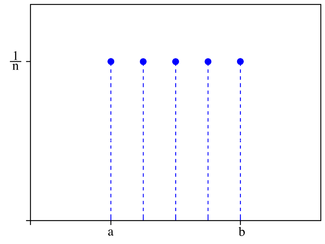
\includegraphics[scale=1]{a_uniform_distribution.png}  
  \caption{ Плотность распределения дискретного равномерного распределения. }
  \label{fig:arch_and_mod:modules:uniform_distribution}
\end{figure}

В зависимости от того, сколько циклов прошло с момента, когда должен был начаться процесс обновления памяти, количество генерируемых адресов, а следовательно количество бит, обращающихся в 0, возрастает по формуле:

\begin{equation}
  \label{eq:arch_and_mod:memory_discharge:e_func}
  f(t) = e^{\frac{\sqrt{t}}
           {5.2}}
\end{equation}

По умолчанию период обновления памяти $T_{refresh}$ = 2600 циклов. 1 цикл равен 3 нсек. Таким образом каждые 7800 нсек память должна обновляться. В итоге в соответствии с формулой примерно через 2000 циклов(с учетом погрешности генератора адресов, т.к. один и тот же адрес может сгенерироваться несколько раз) все ячейки обернутся в 0, если соответствующий процесс регенерации памяти так и не был запущен. График функции представлен на рисунке ~\ref{fig:arch_and_mod:memory_discharge:efunc_grafic}.

\begin{figure}[ht]
\centering
  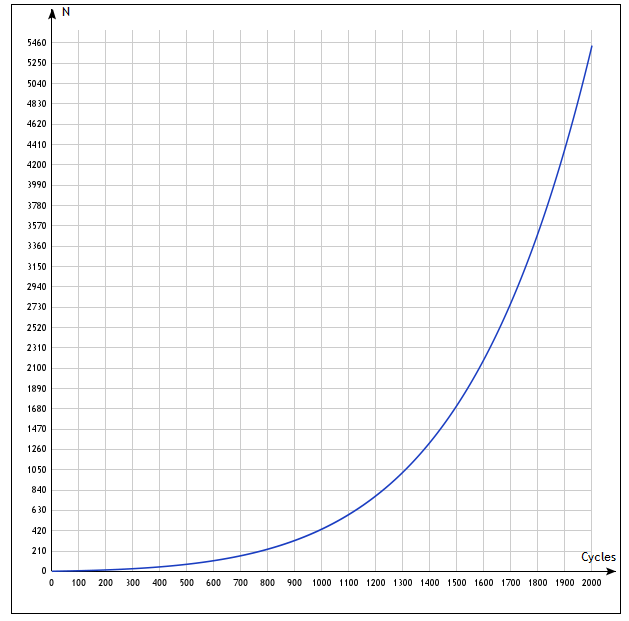
\includegraphics[scale=0.75]{a_efunc.png}  
  \caption{ График экспоненциальной функции ~\ref{eq:arch_and_mod:memory_discharge:e_func} }
  \label{fig:arch_and_mod:memory_discharge:efunc_grafic}
\end{figure}

\subsection{Симуляция процесса регенерации памяти}
\label{sub:arch_and_mod:memory_refresh}

Заряд конденсатора динамического ОЗУ со временем уменьшается вследствие утечки, поэтому для сохранения содержимого памяти процесс регенерации каждой ячейки памяти должен производится через определенное время. На время регенерации взаимодействие ОЗУ с внешними устройствами(драйвером) должно быть приостановлено, т.е. путем перевода этих устройств в режим ожидания.

В первую очередь необходимо выяснить, произошли ли ошибки во время работы памяти. Наиболее экономичным по временным затратам и эффективным методом является алгоритм адаптивного сжатия выходных данных (АСВД) (Self-Adjusting Output Data Compression - SAODC). Подробно данная технология рассмотрена в работах \cite{SAODC_Ivaniuk} и ~\cite{SAODC_Yarmolik}. Данный подход позволяет полностью избежать временных издержек для вычисления эталонной сигнатуры. Согласно этой концепции эталонная характеристика (сигнатура) $S_{ref}$ начального содержимого бит-ориентированного ОЗУ вычисляется как сумма по модулю два всех адресов ячеек, содержащих значение 1. Пример вычисления $S_{ref}$ для ОЗУ с 8 ячейками представлен на рисунке~\ref{fig:arch_and_mod:memory_refresh:saodc}.

\begin{figure}[ht]
\centering
  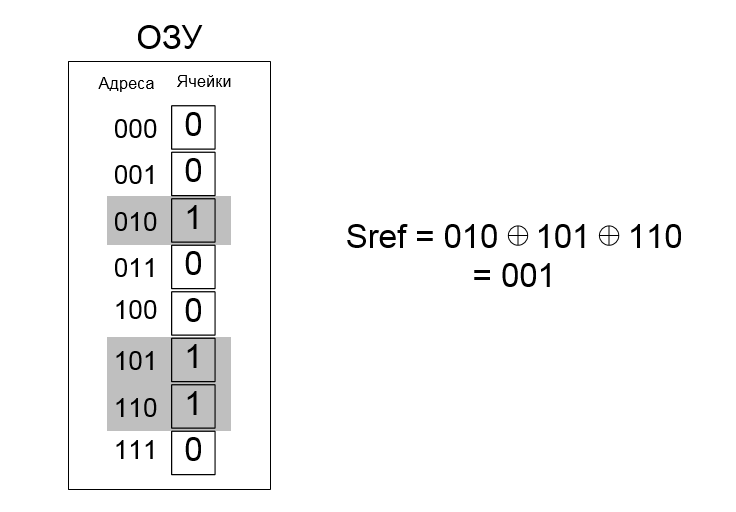
\includegraphics[scale=0.75]{a_saodc.png}  
  \caption{ Вычисление эталонной сигнатуры для бит-ориентированного ОЗУ.}
  \label{fig:arch_and_mod:memory_refresh:saodc}
\end{figure}

При таком методе изменения в памяти не потребуют заново вычислять эталонную сигнатуру, достаточно просто сложить по модулю два адрес изменившейся ячейки со значением эталонной сигнатуры. Обновление сигнатуры выглядит следующим образом:

\begin{equation}
  \label{eq:arch_and_mod:memory_refresh:adjusting_signature}
  S_{ref}^{new} = S_{ref}^{old} \oplus a \cdot ( M[a]^{new} \oplus M[a]^{old} ) \text{\,,}
\end{equation}
\begin{explanation}
где & $ a $ & адрес изменившейся ячейки; \\
    & $ M[a]^{new} $ & новое значение ячейки; \\
    & $ M[a]^{old} $ & старое значение ячейки.
\end{explanation}

Для слово-ориентированного ОЗУ применяется та же схема сжатия данных, но потребуются некоторые дополнительные действия. Пусть имеется память с матрицей ячеек 16 на 16. Т.е. 16 рядов и 16 колонок. Каждая ячейка имеет объём 8 бит. Применяя метод АСА (адаптивный сигнатурный анализатор), теперь нужно оперировать адресами не ячеек, а бит памяти. Таким образом для 5-го бита в ячейке, расположенной на 4-ом ряду и 2-ой колонке адрес будет представлен числом  0x215 в шестнадцатиричной системе счисления, или числом 0100 0010 101 в двоичной. Построение адреса бита пояснено на рисунке ~\ref{fig:arch_and_mod:memory_refresh:address}.

\begin{figure}[ht]
\centering
  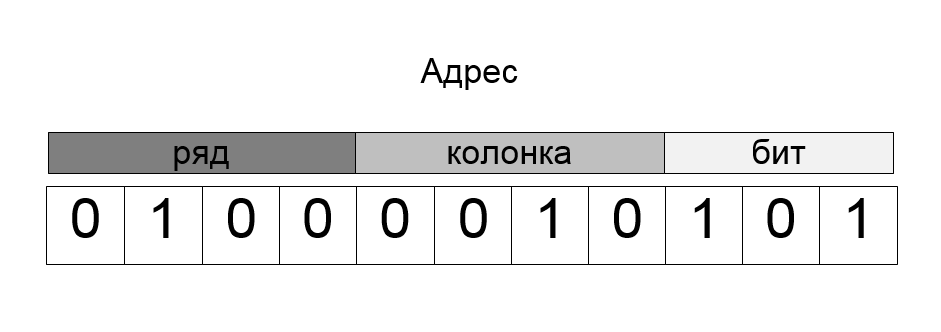
\includegraphics[scale=0.4]{a_address.png}  
  \caption{ Представление адреса бита в слово-ориентированном ОЗУ.}
  \label{fig:arch_and_mod:memory_refresh:address}
\end{figure}

У метода АСА есть недостаток, который заключается в том, что 0-вой адрес ячейки никак не повлияет на общую сумму адресов, т.к. $0 \oplus S = S$. Исходя из этого вместе с данным методом используется также бит четности\cite{March_Tests_Ivaniuk}. Бит четности - это дополнительный бит в младшем разряде адреса ячейки, который всегда содержит 1-цу. Таким образом даже нулевой адрес ячейки повлияет на общую сумму адресов. Но главная особенность бита четности заключается в том, что с его помощью можно определить, какой кратности произошла ошибка. Если тестовая и эталонная сигнатуры не совпали и бит четности равен нулю, тогда произошло четное количество ошибок, в противном случае нечетное.

После каждой операции записи в память, эталонная сигнатура обновляется. При наступлении периода регенерации, высчитывается тестовая сигнатура $S_{test}$ и затем сравнивается с эталонной $S_{ref}$. Если сигнатуры совпали - значит с памятью всё в порядке, в противном случае произошли ошибки. При однократной ошибке достаточно просто найти ядрес ячейки и позицию бита, в котором произошла ошибка. Сложение двух сигнатур  $S_{test} \oplus S_{ref}$ дает адрес бита с изменившимися данными. Таким образом процедура регенерации памяти состоит из следующих шагов:
\begin{enumerate}
  \item При наступлении периода обновления памяти вычисляется тестовая сигнатура и сравнивается с эталонной;
  \item Если сигнатуры не совпали и бит четности равен 1-це, то предполагаем, что произошла однократная ошибка. Инвертируется бит по адресу $S_{test} \oplus S_{ref}$.;
  \item Если сигнатуры не совпали и бит четности равен 0-лю, то произошло четное количество ошибок. Переход к шагу д
  \item Если сигнатуры совпали, то была однократная ошибка, которую удалось устранить. В противном случае переход к шагу д;
  \item Запуск неразрушающего маршевого теста для выявления неисправностей;
  \item Если тест ничего не обнаружил, значит была многократная ошибка, в противном случае неисправность, которую нужно диагностировать;
  \item Повторяется шаг а.
\end{enumerate}

Блок-схема алгоритма регенерации памяти представлена на рисунке ~\ref{fig:arch_and_mod:memory_refresh:refresh_chart}.

\begin{figure}[ht]
\centering
  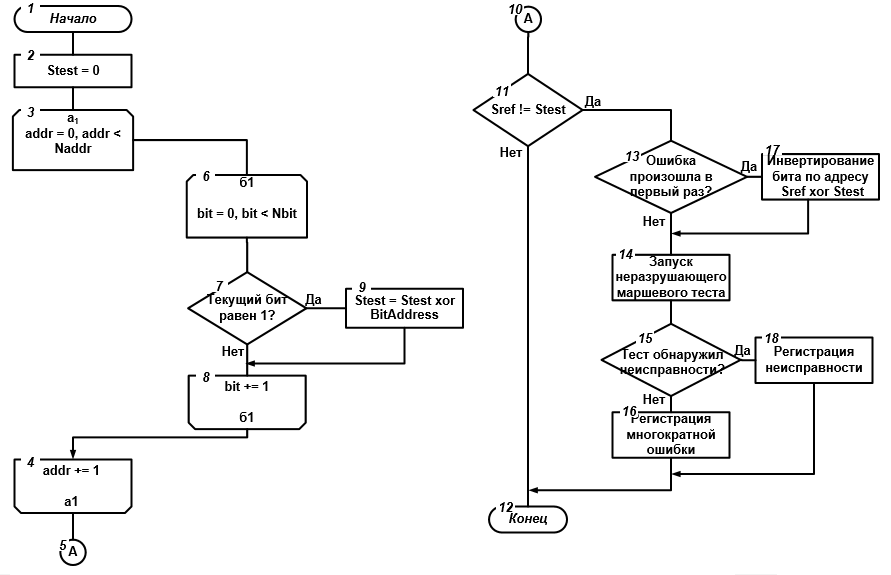
\includegraphics[scale=0.70]{a_refresh_chart.png}  
  \caption{ Схема алгоритма регенерации памяти ОЗУ.}
  \label{fig:arch_and_mod:memory_refresh:refresh_chart}
\end{figure}

За регенерацию памяти отвечает класс RegenerationController. Класс SAODCController обеспечивает вычисление рабочей и эталонной сигнатур. Метод обновления эталонной сигнатуры при каждой операции чтения представлен в листинге ~\ref{lst:arch_and_mod:memory_refresh:update_sig}

\begin{lstlisting}[style=cplusplusstyle, caption={Обновление эталонной сигнатуры ОЗУ}, label=lst:arch_and_mod:memory_refresh:update_sig]
void SAODCController::UpdateRef(BusPacket* packet)
{
    if (packet->busPacketType == DATA)
    {
        uint16_t oldData = dramDevice->read(packet->address);
        uint16_t newData = packet->data->getData();
        if (oldData != newData)
        {
            int address = GetAddress(packet->address, data);
            RefSignature ^= address;       
        }
    }
}

int SAODCController::GetAddress(int rank, int bank, int row, int col, uint16_t data)
{
    //get 'bit address sum'
    if (!data) return 0;
    
    int bitSum = 0;
    int bitCount  = 0; // '1' bit count
    for (int i = 0; (unsigned)i < DEVICE_WIDTH; i++)
    {
        if (data & (1 << i))
        {
            bitSum ^= i;
            bitCount++;
        }
    }
    if (bitCount % 2 == 0)
    addr.Clear();
    
    addr.bit = bitSum;
    int address = addr.GetPhysical();

    if (bitCount % 2 != 0)
        AddParityBit(address);
  
    return address;
}
\end{lstlisting} 

\subsection{Представление маршевых тестов}
\label{sub:arch_and_mod:march_tests}

Для выявления неисправностей ОЗУ решено использовать маршевые тесты из-за их простоты и эффективности. Все маршевые тесты построены по единому принципу и различаются лишь набором элементов. Поэтому целесообразно представить такие тесты с помощью обобщенной структуры, которая может подстроиться под любой тест. Направление перебора адресов отражается элементами MD\_UP, MD\_DOWN и MD\_BOTH перечисления MarchDirection. Операции чтения и записи также представлены элементами перечисления MarchOperation. Элементы MO\_RD и MO\_RDC обозначают операцию чтения прямого и обратного значения в буфер из ячейки памяти, элементы MO\_WD и MO\_WDC описывают операции записи прямого и обратного значения из буфера в ячейку памяти. Фаза маршевого теста отражена в структуре MarchPhase, представленной в листинге ~\ref{lst:arch_and_mod:march_tests:march_phase}.

\begin{lstlisting}[style=cplusplusstyle, caption={Структура фазы маршевого теста}, label=lst:arch_and_mod:march_tests:march_phase]
struct MarchPhase
{
    MarchDirection direction;
    std::vector<MarchOperation> elements;
};
\end{lstlisting} 

Таким образом маршевый тест представляется вектором, содержащим определённое количество структур MarchPhase. Инициализация вектора элементов маршевого теста March C- представлена в листинге ~\ref{lst:arch_and_mod:march_tests:march_init}.

\begin{lstlisting}[style=cplusplusstyle, caption={Инициализация вектора элементов маршевого теста March C-}, label=lst:arch_and_mod:march_tests:march_init]
void InitializeTest()
{
    std::vector<MarchPhase> phases;
    phases.push_back({ MD_UP, { MO_RD, MO_WDC } });
    phases.push_back({ MD_UP, { MO_RDC, MO_WD } });
    phases.push_back({ MD_DOWN, { MO_RD, MO_WDC } });
    phases.push_back({ MD_DOWN, { MO_RDC, MO_WD } });
    phases.push_back({ MD_DOWN, { MO_RD } });
};
\end{lstlisting} 

Другие виды маршевых тестов инициализируются подобным образом. Программа поддерживает следующие маршевые тесты: March C-, March A, March B, March X, March Y, MATS, MATS+, MATS++.

Логика создания и выполнения маршевых тестов находится в классе MarchTestController. Запуск теста производит класс RegenerationController. Для сжатия данных используется адаптивный сигнатурный анализатор, рассмотренный в предыдущем пункте. На этапе инициализации теста в качестве эталонной сигнатуры берётся уже вычисленная ранее рабочая сигнатура класса RegenerationController. Далее на каждой фазе маршевого теста вычисляется тестовая сигнатура и в конце фазы сравнивается с эталонной. При правильном функционировании памяти сигнатуры должны всегда совпадать вне зависимости от операций, производимых элементами маршевого теста. Это происходит потому, что маршевый тест является неразрушающим, а также благодаря свойству АСА, которое заключается в равенстве сумм адресов ячеек, содержащих 1, и адресов ячеек, содержащих 0. Выполнение маршевого теста занимает определённое время, а потому выполнение отдельных его фаз разбито на несколько циклов работы симулятора. Выполнение теста приводится в листинге ~\ref{lst:arch_and_mod:march_tests:march_run}.

\begin{lstlisting}[style=cplusplusstyle, caption={Функция выполнения маршевого теста}, label=lst:arch_and_mod:march_tests:march_run]
void MarchTestController::Update()
{
    if (!state.testStarted) return;

    saodc.ClearTestSig();
    MarchPhase& phase = phases[state.phase];
    int addrStart = 0;
    int counter = 0;
    int bottom = 0;
    int top = NUM_BANKS * NUM_COLS * NUM_ROWS - 1;

    if (phase.direction == MD_UP || phase.direction == MD_BOTH)
    {
        addrStart = bottom;
        counter = 1;
    }
    else if (phase.direction == MD_DOWN)
    {
        addrStart = top;
        counter = -1;
    }
    for (int addr = addrStart; addr >= bottom && addr <= top; addr += counter)
    {
        uint16_t buffer = 0;
        uint16_t old = 0;
        for (auto& el : phase.elements)
        {
            RunElement(el, addr, buffer, old);
        }
    }
    int err = saodc.Compare();
    if (err)
    {
        state.testPassed = false;
        cout << "[MarchTest] Errors are detected while running phase! Signature sum is " << err << "(" << addrTranslator.GetDescription(err, true) << ")" << endl;
    }
    state.phase++;
    if (state.phase == phases.size())
    {
        state.testCompleted = true;
        state.testStarted = false;
    }
}
\end{lstlisting} 

Выполнение каждой отдельной операции маршевого элемента приведено в листинге ~\ref{lst:arch_and_mod:march_tests:march_element_run}.

\begin{lstlisting}[style=cplusplusstyle, caption={Выполнение элемента маршевого теста}, label=lst:arch_and_mod:march_tests:march_element_run]
void MarchTestController::RunElement(int element, int address, uint16_t &buffer, uint16_t& oldValue)
{
    int r = 0, b = 0, row = 0, col = 0;
    addrTranslator.Translate(address, r, b, row, col);
    uint16_t data = 0;
    switch (element)
    {
    case MO_RD:
        data = dramDevice->read(r, b, row, col);
        buffer = data;
        break;
    case MO_RDC:
        data = dramDevice->read(r, b, row, col);
        buffer = ~data;
        break;
    case MO_WD:
        dramDevice->write(r, b, row, col, buffer);
        break;
    case MO_WDC:
        dramDevice->write(r, b, row, col, ~buffer);
        break;
    }
    //convertData
    if (element == MO_RD || element == MO_RDC)
    {
        saodc.UpdateTestSig(addr, data ^ oldValue);
        oldValue = data;
    }
}
\end{lstlisting} 

\subsection{Моделирование функциональных неисправностей ОЗУ}
\label{sub:arch_and_mod:faults}

Для моделирования функциональных неисправностей ОЗУ используется обобщенная структура Fault, представленная в листинге~\ref{lst:arch_and_mod:faults:faults_struct}. 
\begin{lstlisting}[style=cplusplusstyle, caption={Структура описания функциональной неисправности ОЗУ}, label=lst:arch_and_mod:faults:faults_struct]
struct Fault
{
    FaultType type;
    uint16_t victimVal;
    uint16_t agressorVal;
    int agressorAddr;
};
\end{lstlisting} 

Поле type может принимать одно из следующих значений: SAF,TF, AF, CFin, CFid, CFst. Они объединены в перечислении FaultType. Поле victimVal для разных моделей неисправностей имеет различное значение, но обобщенно оно хранит значение ячейки-жертвы. Так для неисправностей типа SAF victimVal будет содержать значение ячейки памяти, которое эта ячейка хранит постоянно и изменить его не может. Для неисправности TF это поле хранит значение, перейдя в которое ячейка превращается в константную, т.е. не может поменять своё состояние. Для неисправностей CFid и CFst данное поле хранит значение, в которое зависимая ячейка принудительно переходит (для CFid) или в которое она может перейти только при определённом значении в ячейке-агрессоре (для CFst). Для неисправностей типа CFin и AF данное поле не неиспользуется. 

Поле agressorAddr хранит адрес ячейки-агрессора. Это поле используется в неисправностях типа CF и AF. Поле agressorVal используется только для CF. Поле agressorVal хранит значение ячейки-агрессора, при котором зависимая ячейка может перейти в состояние victimVal (для CFst) или значение, при переходе в которое, ячейка-жертва насильно меняет своё значение на victimVal (для CFin и CFid). Для неисправности типа AF поле agressorAddr хранит адрес ячейки, при записи значения в которую записываемое значение дублируется по адресу ячейки-жертвы.

Класс, контролирующий поведение ячеек в соответствии с различными моделями неисправностей, называется FaultController и находится в классе DRAMDevice. При каждой операции записи в память FaultController вмешивается в работу системы и имитирует поведение неисправностей. Все основные виды неисправностей выявляются на протяжении работы симулятора, однако при неисправностях типа SAF необходимо инициализировать значения ячеек памяти на старте симулятора. 

Метод, анализирующий операцию записи в ячейку памяти и принимающий решение о выполнении тех или иных действий, соответствующих моделям неисправностей, представлен в листинге~\ref{lst:arch_and_mod:faults:faults_run}.

\begin{lstlisting}[style=cplusplusstyle, caption={Реализаия поведения ячеек с функциональными неисправностями}, label=lst:arch_and_mod:faults:faults_run]
void FaultController::DoFaults(Address addr, uint16_t data)
{
    uint16_t oldData = dramDevice->read(addr);
    uint16_t bitMask = oldData ^ data;
  
    for (unsigned i = 0; i < DEVICE_WIDTH; i++)
    {
        if (bitMask & (1 << i))
        {
            addr.bit = i;
            DoOperationOnBit(addr, data & (1 << i) ? 1 : 0, oldData & (1 << i) ? 1 : 0);
        }
    }
}

void FaultController::DoOperationOnBit(Address address, uint16_t newVal, uint16_t oldVal)
{
    int addr = address.GetPhysical();
    if (IsFaulty(addr))
    {
        Fault fault = GetCellAttributes(addr, false);
        switch (fault.type)
        {
            case SAF: break;
            case TF:
            {
                if (oldVal != fault.victimValue)
                {
                    WriteBit(address, newVal);
                }
                break;
            }
            case CFin:
            {
                WriteBit(address, newVal);
                break;
            }     
            case CFid:
            {
                WriteBit(address, newVal);
                break;
            }
            case CFst:
            {
                if (newVal != fault.victimValue)
                    WriteBit(address, newVal);
                else
                {
                    Address agrAdr(fault.agressorAddress, true);
                    if (dramDevice->readBit(agrAdr) == fault.agressorValue)
                        WriteBit(address, newVal);
                }
                break;
            }
            default: break;
        }
    }
    else
    {
        if (IsAgressor(addr))
        {
            Fault fault = GetCellAttributes(addr, true);      
            switch (fault.type)
            {
                case CFin:
                {
                    if (newVal == fault.agressorValue && newVal != oldVal)
                    {
                        Address vicAdr(fault.victimAddress, true);
                        (*dramDevice->ranks)[vicAdr.rank].banks[vicAdr.bank].invertBit(vicAdr);
                    }
                    break;
                }
                case CFid:
                {
                    if (newVal == fault.agressorValue && newVal != oldVal)
                    {
                        Address vicAdr(fault.victimAddress, true);
                        WriteBit(vicAdr, fault.victimValue);
                    }
                    break;
                }
                case AF:
                {
                    Address vicAdr(fault.victimAddress, true);
                    WriteBit(vicAdr, newVal);
                    break;
                }
                default :
                  break;
            }
            WriteBit(address, newVal);
        }
        else
        {
            WriteBit(address, newVal);
        }
    } 
}
\end{lstlisting} 


\subsection{Верификация неразрушающих маршевых тестов}
\label{sub:arch_and_mod:verification}

Для верификации были взяты следующие неразрушающие маршевые тесты: March C-, March A, March B, March X, March Y, MATS, MATS+, MATS++. Описание тестов находится в таблице \ref{table:arch_and_mod:verification:march_tests}.


\begin{table}[ht]
  \caption{Неразрушающие маршевые тесты}
  \label{table:arch_and_mod:verification:march_tests}
  \begin{tabular}{| >{\centering}m{0.15\textwidth}
                  | >{\centering}m{0.15\textwidth}
                  | >{\centering\arraybackslash}m{0.6\textwidth}|}
   \hline 
  {Название} & {Сложность} & {Описание теста} \\ \hline
   March C- & 9N & $\{\Uparrow (rd,wdc); \Uparrow (rdc,wd); \Downarrow (rd,wdc); \Downarrow (rdc,wd); \Updownarrow (rd)\}$ \\ \hline
   March A & 14N & $\{\Uparrow(rd,wdc,wd,wdc); \Uparrow (rdc,wd,wdc); \Downarrow (rdc,wd,wdc,wd); \Downarrow (rd,wdc,wd)\}$ \\ \hline
   March B & 16N & $\{\Uparrow(rd,wdc,rdc,wd,rd,wdc); \Uparrow (rdc,wd,wdc); \Downarrow (rdc,wd,wdc,wd); \Downarrow (rd,wdc,wd)\}$ \\ \hline
   March X & 5N & $\{\Uparrow (rd,wdc); \Downarrow (rdc,wd); \Updownarrow (rd)\}$ \\ \hline
   March Y & 5N & $\{\Uparrow (rd,wdc,rdc); \Downarrow (rdc,wd,rd); \Updownarrow (rd)\}$ \\ \hline
   MATS & 3N & $\{\Updownarrow (rd,wdc); \Updownarrow (rdc)\}$ \\ \hline
   MATS+ & 4N & $\{\Uparrow (rd,wdc); \Downarrow (rdc,wd)\}$ \\ \hline
   MATS++ & 5N & $\{\Uparrow (rd,wdc); \Downarrow (rdc,wd,rd)\}$ \\ \hline   
  \end{tabular}
\end{table}

Для верификации потребовалось запустить каждый тест для каждой модели неисправности, находящейся в памяти. Всего были проверены 26 неисправностей: 2 вида SAF, 2 вида TF, 2 вида AF, 4 вида CFin, 8 видов CFid и 8 видов CFst. В качестве неисправностей AF были взяты только два случая: когда адрес ячейки, чье значение при записи дублируется в ячейку-жерту, меньше, чем адрес ячейки-жертвы, и наоборот. 

Для неисправностей SAF, TF, AF и CFin результаты тестов приведены в таблице \ref{table:arch_and_mod:verification:coverage1}.

\begin{table}[!ht]
\caption{Покрывающая способность неразрушающих маршевых тестов неисправностей SAF, TF, AF и CFin}
\label{table:arch_and_mod:verification:coverage1}
  \centering
  \begin{tabular}{| >{\centering}m{0.13\textwidth} 
                  | >{\centering}m{0.02\textwidth} 
                  | >{\centering}m{0.02\textwidth} 
                  | >{\centering}m{0.02\textwidth} 
                  | >{\centering}m{0.02\textwidth} 
                  | >{\centering}m{0.05\textwidth} 
                  | >{\centering}m{0.05\textwidth} 
                  | >{\centering}m{0.1\textwidth} 
                  | >{\centering}m{0.1\textwidth} 
                  | >{\centering}m{0.1\textwidth} 
                  | >{\centering\arraybackslash}m{0.1\textwidth}|}
    \hline
    \multirow{3}{0.13\textwidth}{\centering Тест} & \multicolumn{10}{c|}{Модели неисправностей} \\ \cline{2-11}    
    & \multicolumn{2}{c|}{SAF} & \multicolumn{2}{c|}{TF} & \multicolumn{2}{c|}{AF} & \multicolumn{4}{c|}{CFin} \\ \cline{2-11}
    & 0 & 1 & $\downarrow$ & $\uparrow$ & $\wedge(b)$ & $\vee(b)$ & $\wedge(\uparrow,b)$ & $\wedge(\downarrow,b)$ & $\vee(\uparrow,b)$ & $\vee(\downarrow,b)$ \\ \hline
    
    March C-  & + & + & + & + & + & + & + & + & + & +\\ \hline
    March A   & + & + & + & + & + & + & + & + & + & +\\ \hline
    March B   & + & + & + & + & + & + & + & + & + & +\\ \hline
    March X   & + & + & + & + & + & + & + & + & + & +\\ \hline
    March Y   & + & + & + & + & + & + & + & + & + & +\\ \hline
    MATS      & + & + & + & - & + & - & + & - & + & -\\ \hline
    MATS+     & + & + & + & - & + & + & + & - & + & +\\ \hline
    MATS++    & - & - & - & + & + & + & + & - & + & +\\ \hline
  \end{tabular}
\end{table}

Для неисправностей CFid результаты тестов приведены в таблице \ref{table:arch_and_mod:verification:coverage2}.

\begin{table}[!ht]
\caption{Покрывающая способность неразрушающих маршевых тестов неисправностей CFid}
\label{table:arch_and_mod:verification:coverage2}
  \centering
  \begin{tabular}{| >{\centering}m{0.12\textwidth} 
                  | >{\centering}m{0.075\textwidth} 
                  | >{\centering}m{0.075\textwidth} 
                  | >{\centering}m{0.075\textwidth} 
                  | >{\centering}m{0.075\textwidth} 
                  | >{\centering}m{0.075\textwidth} 
                  | >{\centering}m{0.075\textwidth} 
                  | >{\centering}m{0.075\textwidth} 
                  | >{\centering\arraybackslash}m{0.1\textwidth}|}
    \hline
    \multirow{3}{0.12\textwidth}{\centering Тест} & \multicolumn{8}{c|}{Модели неисправностей} \\ \cline{2-9}    
    & \multicolumn{8}{c|}{CFid} \\ \cline{2-9}
    & {$\wedge$ \\ $(\uparrow,0)$} & {$\wedge$ \\ $(\uparrow,1)$} & {$\wedge$ \\ $(\downarrow,0)$} & {$\wedge$ \\ $(\downarrow,1)$} 
    & {$\vee$ \\ $(\uparrow,0)$} & {$\vee$ \\ $(\uparrow,1)$} & {$\vee$ \\ $(\downarrow,0)$} & $\vee(\downarrow,1)$ \\ \hline
    
    March C-  & + & + & + & + & + & + & + & + \\ \hline
    March A   & + & + & + & + & + & + & + & + \\ \hline
    March B   & + & + & + & + & + & + & + & + \\ \hline
    March X   & - & + & - & + & + & - & + & - \\ \hline
    March Y   & - & + & - & + & + & - & + & - \\ \hline
    MATS      & - & + & - & - & + & - & - & - \\ \hline
    MATS+     & - & + & - & - & + & - & + & - \\ \hline
    MATS++    & - & + & - & - & + & - & + & - \\ \hline
  \end{tabular}
\end{table}

Для неисправностей CFst результаты тестов приведены в таблице \ref{table:arch_and_mod:verification:coverage3}.

\begin{table}[!ht]
\caption{Покрывающая способность неразрушающих маршевых тестов неисправностей CFst}
\label{table:arch_and_mod:verification:coverage3}
  \centering
  \begin{tabular}{| >{\centering}m{0.12\textwidth} 
                  | >{\centering}m{0.075\textwidth} 
                  | >{\centering}m{0.075\textwidth} 
                  | >{\centering}m{0.075\textwidth} 
                  | >{\centering}m{0.075\textwidth} 
                  | >{\centering}m{0.075\textwidth} 
                  | >{\centering}m{0.075\textwidth} 
                  | >{\centering}m{0.075\textwidth} 
                  | >{\centering\arraybackslash}m{0.1\textwidth}|}
    \hline
    \multirow{3}{0.12\textwidth}{\centering Тест} & \multicolumn{8}{c|}{Модели неисправностей} \\ \cline{2-9}    
    & \multicolumn{8}{c|}{CFst} \\ \cline{2-9}
    & {$\wedge$ \\ $(0,0)$} & {$\wedge$ \\ $(0,1)$} & {$\wedge$ \\ $(1,0)$} & {$\wedge$ \\ $(1,1)$} 
    & {$\vee$ \\ $(0,0)$} & {$\vee$ \\ $(0,1)$} & {$\vee$ \\ $(1,0)$} & $\vee(1,1)$ \\ \hline
    
    March C-  & + & + & + & + & + & + & + & + \\ \hline
    March A   & + & + & - & - & - & + & + & + \\ \hline
    March B   & + & + & - & - & - & + & + & + \\ \hline
    March X   & + & + & - & - & - & - & + & + \\ \hline
    March Y   & + & + & - & - & - & - & + & + \\ \hline
    MATS      & - & + & - & - & - & - & - & + \\ \hline
    MATS+     & - & + & - & - & - & - & - & + \\ \hline
    MATS++    & + & - & - & - & - & - & + & - \\ \hline
  \end{tabular}
\end{table}

Обобщенные результаты по всем тестам представлены в таблице\ref{table:arch_and_mod:verification:coverage}.

\begin{table}[!ht]
\caption{Покрывающая способность неразрушающих маршевых тестов}
\label{table:arch_and_mod:verification:coverage}
  \centering
  \begin{tabular}{| >{\centering}m{0.2\textwidth} 
                  | >{\centering}m{0.1\textwidth} 
                  | >{\centering}m{0.1\textwidth} 
                  | >{\centering}m{0.1\textwidth} 
                  | >{\centering}m{0.1\textwidth} 
                  | >{\centering}m{0.1\textwidth} 
                  | >{\centering\arraybackslash}m{0.1\textwidth}|}
    \hline
    \multirow{2}{0.15\textwidth}{\centering Тест} &
    \multicolumn{6}{c|}{\centering Модели неисправностей} \\
    \cline{2-7}
    & SAF & TF & AF & CFin & CFid & CFst \\
    \hline
     March C-   & 2/2 & 2/2 & 2/2 & 4/4 & 8/8 & 8/8 \\ \hline
     March A    & 2/2 & 2/2 & 2/2 & 4/4 & 8/8 & 5/8 \\ \hline
     March B    & 2/2 & 2/2 & 2/2 & 4/4 & 8/8 & 5/8 \\ \hline
     March X    & 2/2 & 2/2 & 2/2 & 4/4 & 4/8 & 4/8 \\ \hline
     March Y    & 2/2 & 2/2 & 2/2 & 4/4 & 4/8 & 4/8 \\ \hline
     MATS       & 2/2 & 1/2 & 1/2 & 2/4 & 2/8 & 2/8 \\ \hline
     MATS+      & 2/2 & 1/2 & 2/2 & 3/4 & 3/8 & 2/8 \\ \hline
     MATS++     & 0/2 & 1/2 & 2/2 & 3/4 & 3/8 & 2/8 \\ \hline
  \end{tabular}
\end{table}

Из результатов тестов видно, что наибольшей покрывающей способностью обладает маршевый тест March C-. По сравнению с тестами March A и March B, которые также имеют хорошие показатели обнаружения неисправностей, тест March C- не только охватывает больше неисправностей, но и является оптимальным по скорости по сравнению с предыдущими тестами. 







%\newcommand{\byr}{Br}

\section{Технико-экономическое обоснование разработки ПС}

% Begin Calculations

\FPeval{\totalProgramSize}{15150}
\FPeval{\totalProgramSizeCorrected}{6550}

\FPeval{\normativeManDays}{172} %Tn

\FPeval{\additionalComplexity}{0.12} %Ksl
\FPeval{\complexityFactor}{clip(1 + \additionalComplexity)}

\FPeval{\stdModuleUsageFactor}{0.7} %Kt
\FPeval{\originalityFactor}{0.7} %Kn

\FPeval{\adjustedManDaysExact}{clip( \normativeManDays * \complexityFactor * \stdModuleUsageFactor * \originalityFactor )}
\FPround{\adjustedManDays}{\adjustedManDaysExact}{0}

\FPeval{\daysInYear}{366}
\FPeval{\redLettersDaysInYear}{6}
\FPeval{\weekendDaysInYear}{105}
\FPeval{\vocationDaysInYear}{24}
\FPeval{\workingDaysInYear}{ clip( \daysInYear - \redLettersDaysInYear - \weekendDaysInYear - \vocationDaysInYear ) }

\FPeval{\developmentTimeMonths}{3}
\FPeval{\developmentTimeYearsExact}{clip(\developmentTimeMonths / 12)}
\FPround{\developmentTimeYears}{\developmentTimeYearsExact}{2}
\FPeval{\requiredNumberOfProgrammersExact}{ clip( \adjustedManDays / (\developmentTimeYears * \workingDaysInYear) + 0.5 ) }

% тут должно получаться 2 ))
\FPtrunc{\requiredNumberOfProgrammers}{\requiredNumberOfProgrammersExact}{0}

\FPeval{\tariffRateFirst}{298000} %Tm1
\FPeval{\tariffFactorFst}{3.04}
\FPeval{\tariffFactorSnd}{3.48}


\FPeval{\employmentFstExact}{clip( \adjustedManDays / \requiredNumberOfProgrammers )}
\FPtrunc{\employmentFst}{\employmentFstExact}{0}

\FPeval{\employmentSnd}{clip(\adjustedManDays - \employmentFst)}


\FPeval{\workingHoursInMonth}{160} %Fr
\FPeval{\salaryPerHourFstExact}{clip( \tariffRateFirst * \tariffFactorFst / \workingHoursInMonth )}
\FPeval{\salaryPerHourSndExact}{clip( \tariffRateFirst * \tariffFactorSnd / \workingHoursInMonth )}
\FPround{\salaryPerHourFst}{\salaryPerHourFstExact}{0}
\FPround{\salaryPerHourSnd}{\salaryPerHourSndExact}{0}

\FPeval{\bonusRate}{1.5}
\FPeval{\workingHoursInDay}{8}
\FPeval{\totalSalaryExact}{clip( \workingHoursInDay * \bonusRate * ( \salaryPerHourFst * \employmentFst + \salaryPerHourSnd * \employmentSnd ) )}
\FPround{\totalSalary}{\totalSalaryExact}{0}

\FPeval{\additionalSalaryNormative}{20}

\FPeval{\additionalSalaryExact}{clip( \totalSalary * \additionalSalaryNormative / 100 )}
\FPround{\additionalSalary}{\additionalSalaryExact}{0}

\FPeval{\socialNeedsNormative}{0.5}
\FPeval{\socialProtectionNormative}{34}
\FPeval{\socialProtectionFund}{ clip(\socialNeedsNormative + \socialProtectionNormative) }

\FPeval{\socialProtectionCostExact}{clip( (\totalSalary + \additionalSalary) * \socialProtectionFund / 100 )}
\FPround{\socialProtectionCost}{\socialProtectionCostExact}{0}

\FPeval{\stuffNormative}{3}
\FPeval{\stuffCostExact}{clip( \totalSalary * \stuffNormative / 100 )}
\FPround{\stuffCost}{\stuffCostExact}{0}

\FPeval{\timeToDebugCodeNormative}{15}
%\FPeval{\reducingTimeToDebugFactor}{0.3} %?
\FPeval{\adjustedTimeToDebugCodeNormative}{\timeToDebugCodeNormative}

\FPeval{\oneHourMachineTimeCost}{5000}

\FPeval{\machineTimeCostExact}{ clip( \oneHourMachineTimeCost * \totalProgramSizeCorrected / 100 * \adjustedTimeToDebugCodeNormative ) }
\FPround{\machineTimeCost}{\machineTimeCostExact}{0}

\FPeval{\businessTripNormative}{15}
\FPeval{\businessTripCostExact}{ clip( \totalSalary * \businessTripNormative / 100 ) }
\FPround{\businessTripCost}{\businessTripCostExact}{0}

\FPeval{\otherCostNormative}{20}
\FPeval{\otherCostExact}{clip( \totalSalary * \otherCostNormative / 100 )}
\FPround{\otherCost}{\otherCostExact}{0}

\FPeval{\overheadCostNormative}{100}
\FPeval{\overallCostExact}{clip( \totalSalary * \overheadCostNormative / 100 )}
\FPround{\overheadCost}{\overallCostExact}{0}

\FPeval{\overallCost}{clip( \totalSalary + \additionalSalary + \socialProtectionCost + \stuffCost + \machineTimeCost + \businessTripCost + \otherCost + \overheadCost ) } 

\FPeval{\supportNormative}{30}
\FPeval{\softwareSupportCostExact}{clip( \overallCost * \supportNormative / 100 )}
\FPround{\softwareSupportCost}{\softwareSupportCostExact}{0}


\FPeval{\baseCost}{ clip( \overallCost + \softwareSupportCost ) }

\FPeval{\profitability}{35}
\FPeval{\incomeExact}{clip( \baseCost / 100 * \profitability )}
\FPround{\income}{\incomeExact}{0}

\FPeval{\estimatedPrice}{clip( \income + \baseCost )}

\FPeval{\localRepubTaxNormative}{3.9}
\FPeval{\localRepubTaxExact}{clip( \estimatedPrice * \localRepubTaxNormative / (100 - \localRepubTaxNormative) )}
\FPround{\localRepubTax}{\localRepubTaxExact}{0}
%\FPeval{\localRepubTax}{0}

\FPeval{\ndsNormative}{20}
\FPeval{\ndsExact}{clip( (\estimatedPrice + \localRepubTax) / 100 * \ndsNormative )}
\FPround{\nds}{\ndsExact}{0}


\FPeval{\sellingPrice}{clip( \estimatedPrice + \localRepubTax + \nds )}

\FPeval{\taxForIncome}{18}
\FPeval{\incomeWithTaxesExact}{clip(\income * (1 - \taxForIncome / 100))}
\FPround{\incomeWithTaxes}{\incomeWithTaxesExact}{0}

% End Calculations

Целью дипломного проекта является создание программного средства для верификации алгоритмов тестирования оперативных запоминающих устройств.
Данное программное средство позволяет облегчить верификацию ОЗУ, не прибегая к тестированию реальных микросистем. Основными достоинствами программного средства являются: симуляция реальных процессов ОЗУ, что позволяет обеспечить максимальную схожесть с реальными системами на чипе, существенное увелечение удобства процесса запуска и верификации тестов динамической оперативной памяти, актуальность.

В данном разделе рассмотрим экономическую эффективность программного средства. Программный комплекс относится ко 2-ой группе сложности. Категория новизны продукта - «В».
Для оценки экономической эффективности разработанного программного средства проводится расчет цены и прибыли от продажи одной системы(программы).

Расчеты выполнены на основе методического пособия \cite{palicyn_2006}.

\subsection{Расчёт сметы затрат и цены программного продукта}

Целесообразность создания коммерческого ПО требует проведения предварительной экономической оценки и расчета экономического эффекта.
Экономический эффект у разработчика ПО зависит от объёма инвестиций в разработку проекта, цены на готовый программный продукт и количества проданных копий, и проявляется в виде роста чистой прибыли.

Исходные данные для разрабатываемого проекта указаны в таблице \ref{table:econ:initial_data}. На основании сметы затрат и анализа рынка ПО определяется плановая отпускаемая цена.
Расчет объёма программного продукта (количества строк исходного кода) предполагает определение типа программного обеспечения, всестороннее техническое обоснование функций ПО и определение объёма каждой функций.
Согласно классификации типов программного обеспечения \cite[с.~59,~приложение 1]{palicyn_2006}, разрабатываемое ПО с наименьшей ошибкой можно классифицировать как ПО методo"=ориентированных расчетов.

\begin{table}[!ht]
\caption{Исходные данные}
\label{table:econ:initial_data}
  \centering
  \begin{tabular}{| >{\raggedright}m{0.62\textwidth}
                  | >{\centering}m{0.17\textwidth}
                  | >{\centering\arraybackslash}m{0.13\textwidth}|}
    \hline
    {\begin{center}
      Наименование
    \end{center} } & Условное обозначение & Значение \\
    \hline
    Категория сложности & & 2 \\

    \hline
    Коэффициент сложности, ед. & $ \text{К}_\text{с} $ & \num{\complexityFactor} \\

    \hline
    Степень использования при разработке стандартных модулей, ед. & $ \text{К}_\text{т} $ & \num{\stdModuleUsageFactor} \\

    \hline
    Коэффициент новизны, ед. & $ \text{К}_\text{н} $ & \num{\originalityFactor} \\

    \hline
    Годовой эффективный фонд времени, дн. & $ \text{Ф}_\text{эф} $ & \num{\workingDaysInYear} \\

    \hline
    Продолжительность рабочего дня, ч. & $ \text{Т}_\text{ч} $ & \num{\workingHoursInDay} \\

    \hline
    Месячная тарифная ставка первого разряда, \byr{} & $ \text{Т}_{\text{м}_{1}}$ & \num{\tariffRateFirst} \\

    \hline
    Коэффициент премирования, ед. & $ \text{К} $ & \num{\bonusRate} \\

    \hline
    Норматив дополнительной заработной платы, ед. & $ \text{Н}_\text{д} $ & \num{\additionalSalaryNormative} \\

    \hline
    Норматив отчислений в ФСЗН и обязательное страхование, $\%$ & $ \text{Н}_\text{сз} $ & \num{\socialProtectionFund} \\

    \hline
    Норматив командировочных расходов, $\%$ & $ \text{Н}_\text{к} $ & \num{\businessTripNormative} \\

    \hline
    Норматив прочих затрат, $\%$ & $ \text{Н}_\text{пз} $ & \num{\otherCostNormative} \\

    \hline
    Норматив накладных расходов, $\%$ & $ \text{Н}_\text{рн} $ & \num{\overheadCostNormative} \\

    \hline
    Прогнозируемый уровень рентабельности, $\%$ & $ \text{У}_\text{рп} $ & \num{\profitability} \\

    \hline
    Норматив НДС, $\%$ & $ \text{Н}_\text{дс} $ & \num{\ndsNormative} \\

    \hline
    Норматив налога на прибыль, $\%$ & $ \text{Н}_\text{п} $ & \num{\taxForIncome} \\

    \hline
    Норматив расхода материалов, $\%$ & $ \text{Н}_\text{мз} $ & \num{\stuffNormative} \\

    \hline
    Норматив расхода машинного времени, ч. & $ \text{Н}_\text{мв} $ & \num{\adjustedTimeToDebugCodeNormative} \\

    \hline
    Цена одного часа машинного времени, \byr{} & $ \text{Н}_\text{мв} $ & \num{\oneHourMachineTimeCost} \\

    \hline
    Норматив расходов на сопровождение и адаптацию ПО, $\%$ & $ \text{Н}_\text{рса} $ & \num{\supportNormative} \\
    \hline
  \end{tabular}
\end{table}


Общий объём программного продукта определяется исходя из количества и объёма функций, реализованных в программе:
\begin{equation}
  \label{eq:econ:total_program_size}
  V_{o} = \sum_{i = 1}^{n} V_{i} \text{\,,}
\end{equation}
\begin{explanation}
где & $ V_{i} $ & объём отдельной функции ПО, LoC; \\
    & $ n $ & общее число функций.
\end{explanation}

На стадии технико-экономического обоснования проекта рассчитать точный объём функций невозможно.
Вместо вычисления точного объёма функций применяются приблизительные оценки на основе данных по аналогичным проектам или по нормативам \cite[с.~61,~приложение 2]{palicyn_2006}, которые приняты в организации.

\begin{table}[ht]
\caption{Перечень и объём функций программного модуля}
\label{table:econ:function_sizes}
\centering
  \begin{tabular}{| >{\centering}m{0.12\textwidth}
                  | >{\raggedright}m{0.40\textwidth}
                  | >{\centering}m{0.18\textwidth}
                  | >{\centering\arraybackslash}m{0.18\textwidth}|}

  \hline
         \multirow{2}{0.12\textwidth}[-0.5em]{\centering \No{} функции}
       & \multirow{2}{0.40\textwidth}[-0.55em]{\centering Наименование (содержание)}
       & \multicolumn{2}{c|}{\centering Объём функции, LoC} \tabularnewline

  \cline{3-4} &
       & { по каталогу ($ V_{i} $) }
       & { уточненный ($ V_{i}^{\text{у}} $) } \tabularnewline

  \hline
  101 & Организация ввода информации & \num{150} & \num{70} \tabularnewline

  \hline
  102 & Контроль, предварительная обработка и ввод информации & \num{450} & \num{300} \tabularnewline

  \hline
  111 & Управление вводом/выводом & \num{2400} & \num{1000} \tabularnewline

  \hline
  301 & Формирование последовательного файла & \num{290} & \num{250} \tabularnewline

  \hline
  305 & Обработка файлов & \num{420} & \num{350} \tabularnewline

  \hline
  501 & Монитор ПО (управление работой компонентов) & \num{740} & \num{700} \tabularnewline

  \hline
  506 & Обработка ошибочных и сбойных ситуаций & \num{410} & \num{400} \tabularnewline

  \hline
  507 & Обеспечение интерфейса между компонентами & \num{970} & \num{680} \tabularnewline

  \hline
  701 & Математическая статистика и прогнозирование & \num{9320} & \num{2800} \tabularnewline

  \hline

  % Уточенная оценка вычислялась с помощью R: (+ручной фикс)
  % set.seed(35)
  % locs <- c(100, 520, 2700, 520, 750, 1100, 430, 730, 460, 8370)
  % locs.which.corrected <- rbinom(length(locs), 1, 0.4)
  % locs.corrections <- rnorm(length(locs), mean = -0.25, sd=0.3)
  % locs.correction.factor <- 1 + locs.which.corrected * locs.corrections
  % locs.corrected <- signif(locs * locs.correction.factor, digits = 2)
  % locs.corrected
  % sum(locs)
  % sum(locs.corrected)

  Итог & & {\num{\totalProgramSize}} & {\num{\totalProgramSizeCorrected}} \tabularnewline

  \hline

  \end{tabular}
\end{table}

Перечень и объём функций программного модуля перечислен в таблице~\ref{table:econ:function_sizes}.
По приведенным данным уточненный объём некоторых функций изменился, и общий уточненный объём ПО $ V_{\text{у}} = \SI{\totalProgramSizeCorrected}{\text{LoC}} $.

\subsection{Расчёт нормативной трудоемкости}

На основании общего объема ПО определяется нормативная трудоемкость ($ \text{Т}_\text{н}$) с учетом сложности ПО. Для ПО 2-ой группы сложности, к которой относится разрабатываемый программный продукт, нормативная трудоемкость составит~$ \text{Т}_\text{н} = \SI{\normativeManDays}{\text{чел.} / \text{дн.}}  $

Нормативная трудоемкость служит основой для оценки общей трудоемкости~$ \text{Т}_\text{о} $.
Используем формулу (\ref{eq:econ:effort_common}) для оценки общей трудоемкости для небольших проектов:
\begin{equation}
  \label{eq:econ:effort_common}
  \text{Т}_\text{о} = \text{Т}_\text{н} \cdot
                      \text{К}_\text{с} \cdot
                      \text{К}_\text{т} \cdot
                      \text{К}_\text{н} \text{\,,}
\end{equation}
\begin{explanation}
где & $ \text{К}_\text{с} $ & коэффициент, учитывающий сложность ПО; \\
    & $ \text{К}_\text{т} $ & поправочный коэффициент, учитывающий степень использования при разработке стандартных модулей; \\
    & $ \text{К}_\text{н} $ & коэффициент, учитывающий степень новизны ПО.
\end{explanation}

Дополнительные затраты труда на разработку ПО учитываются через коэффициент сложности, который вычисляется по формуле
\begin{equation}
\label{eq:econ:complexity_coeff}
  \text{К}_{\text{с}} = 1 + \sum_{i = 1}^n \text{К}_{i} \text{\,,}
\end{equation}
\begin{explanation}
где & $ \text{К}_{i} $ & коэффициент, соответствующий степени повышения сложности ПО за счет конкретной характеристики; \\
    & $ n $ & количество учитываемых характеристик.
\end{explanation}

Наличие двух характеристик сложности позволяет \cite[c.~66, приложение~4, таблица~П.4.2]{palicyn_2006} вычислить коэффициент сложности
\begin{equation}
\label{eq:econ:complexity_coeff_calc}
  \text{К}_{\text{с}} = \num{1} + \num{\additionalComplexity} = \num{\complexityFactor} \text{\,.}
\end{equation}

Разрабатываемое ПО использует стандартные компоненты. Согласно справочным данным \cite[c.~68,~приложение~4, таблица~П.4.5]{palicyn_2006} коэффициент использования стандартных модулей для разрабатываемого приложения $ \text{К}_\text{т} = \num{\stdModuleUsageFactor} $.
Разрабатываемое ПО не является новым, существуют аналогичные более зрелые разработки у различных компаний и университетов по всему миру.
Влияние степени новизны на трудоемкость создания ПО определяется коэффициентом новизны~---~$ \text{К}_\text{н} $.
Согласно справочным данным \cite[c.~67, приложение~4, таблица~П.4.4]{palicyn_2006} для разрабатываемого ПО $ \text{К}_\text{н} = \num{\originalityFactor} $.
Подставив приведенные выше коэффициенты для разрабатываемого ПО в формулу~(\ref{eq:econ:effort_common}) получим общую трудоемкость разработки
\begin{equation}
  \label{eq:econ:effort_common_calc}
  \text{Т}_\text{о} = \num{\normativeManDays} \cdot \num{\complexityFactor} \cdot \num{\stdModuleUsageFactor} \cdot \num{\originalityFactor} \approx \SI{\adjustedManDays}{\text{чел.}/\text{дн.}}
\end{equation}

На основе общей трудоемкости и требуемых сроков реализации проекта вычисляется плановое количество исполнителей.
Численность исполнителей проекта рассчитывается по формуле:
\begin{equation}
  \label{eq:econ:num_of_programmers}
  \text{Ч}_\text{р} = \frac{\text{Т}_\text{о}}{\text{Т}_\text{р} \cdot \text{Ф}_\text{эф}} \text{\,,}
\end{equation}
\begin{explanation}
где & $ \text{Т}_\text{о} $ & общая трудоемкость разработки проекта, $ \text{чел.}/\text{дн.} $; \\
    & $ \text{Ф}_\text{эф} $ & эффективный фонд времени работы одного работника в течение года, дн.; \\
    & $ \text{Т}_\text{р} $ & срок разработки проекта, лет.
\end{explanation}

Эффективный фонд времени работы одного разработчика вычисляется по следующей формуле:
\begin{equation}
  \label{eq:econ:effective_time_per_programmer}
  \text{Ф}_\text{эф} =
    \text{Д}_\text{г} -
    \text{Д}_\text{п} -
    \text{Д}_\text{в} -
    \text{Д}_\text{о} \text{\,,}
\end{equation}
\begin{explanation}
где & $ \text{Д}_\text{г} $ & количество дней в году, дн.; \\
    & $ \text{Д}_\text{п} $ & количество праздничных дней в году, не совпадающих с выходными днями, дн.; \\
    & $ \text{Д}_\text{в} $ & количество выходных дней в году, дн.; \\
    & $ \text{Д}_\text{п} $ & количество дней отпуска, дн.
\end{explanation}

Согласно данным, приведенным в производственном календаре для пятидневной рабочей недели в 2016 году для Беларуси \cite{belcalendar_2016}, фонд рабочего времени составит
\begin{equation}
  \text{Ф}_\text{эф} = \num{\daysInYear} - \num{\redLettersDaysInYear} - \num{\weekendDaysInYear} - \num{\vocationDaysInYear} = \SI{\workingDaysInYear}{\text{дн.}}
\end{equation}

Учитывая срок разработки проекта $ \text{Т}_\text{р} = \SI{\developmentTimeMonths}{\text{мес.}} = \SI{\developmentTimeYears}{\text{года}} $, общую трудоемкость и фонд эффективного времени одного работника, вычисленные ранее, можем рассчитать численность исполнителей проекта
\begin{equation}
  \label{eq:econ:num_of_programmers_calc}
  \text{Ч}_\text{р} =
    \frac{\num{\adjustedManDays}}
         {\num{\developmentTimeYears} \cdot \num{\workingDaysInYear}}
    \approx \SI{\requiredNumberOfProgrammers}{\text{рабочих}}.
\end{equation}

Вычисленные оценки показывают, что для выполнения запланированного проекта в указанные сроки необходимо два рабочих.

\subsection{Расчёт основной заработной платы исполнителей}

Информация о работниках перечислена в таблице~\ref{table:econ:programmers}.
\begin{table}[ht]
  \caption{Работники, занятые в проекте}
  \label{table:econ:programmers}
  \begin{tabular}{| >{\centering}m{0.4\textwidth}
                  | >{\centering}m{0.15\textwidth}
                  | >{\centering}m{0.18\textwidth}
                  | >{\centering\arraybackslash}m{0.15\textwidth}|}
   \hline
   Исполнители & Разряд & Тарифный коэффициент & \mbox{Чел./дн.} занятости \\
   \hline
   Программист \Rmnum{1}-категории & $ \num{13} $ & $ \num{\tariffFactorFst} $ & $ \num{\employmentFst} $ \\
   \hline
   Ведущий программист & $ \num{15} $ & $ \num{\tariffFactorSnd} $ & $ \num{\employmentSnd} $ \\
   \hline
  \end{tabular}
\end{table}

Месячная тарифная ставка одного работника вычисляется по формуле
\begin{equation}
  \label{eq:econ:month_salary}
  \text{Т}_\text{ч} =
    \frac {\text{Т}_{\text{м}_{1}} \cdot \text{Т}_{\text{к}} }
          {\text{Ф}_{\text{р}} }  \text{\,,}
\end{equation}
\begin{explanation}
где & $ \text{Т}_{\text{м}_{1}} $ & месячная тарифная ставка 1-го разряда, \byr; \\
    & $ \text{Т}_{\text{к}} $ & тарифный коэффициент, соответствующий установленному тарифному разряду; \\
    & $ \text{Ф}_{\text{р}} $ & среднемесячная норма рабочего времени, час.
\end{explanation}




Подставив данные из таблицы~\ref{table:econ:programmers} в формулу~(\ref{eq:econ:month_salary}), приняв значение тарифной ставки 1-го разряда $ \text{Т}_{\text{м}_{1}} = \SI{\tariffRateFirst}{\text{\byr}} $ и среднемесячную норму рабочего времени $ \text{Ф}_{\text{р}} = \SI{\workingHoursInMonth}{\text{часов}} $ получаем:
\begin{equation}
  \label{eq:econ:month_salary_calc1}
  \text{Т}_{\text{ч}}^{\text{прогр. \Rmnum{1}-разр.}} = \frac{ \num{\tariffRateFirst} \cdot \num{\tariffFactorFst} } { \num{\workingHoursInMonth} } = \SI{\salaryPerHourFst}{\text{\byr}/\text{час;}}
\end{equation}
\begin{equation}
  \label{eq:econ:month_salary_calc2}
  \text{Т}_{\text{ч}}^{\text{вед. прогр.}} = \frac{ \num{\tariffRateFirst} \cdot \num{\tariffFactorSnd} } { \num{\workingHoursInMonth} } = \SI{\salaryPerHourSnd}{\text{\byr}/\text{час.}}
\end{equation}

Основная заработная плата исполнителей на конкретное ПО рассчитывается по формуле:
\begin{equation}
  \label{eq:econ:total_salary}
  \text{З}_{\text{о}} = \sum^{n}_{i = 1}
                        \text{Т}_{\text{ч}}^{i} \cdot
                        \text{Т}_{\text{ч}} \cdot
                        \text{Ф}_{\text{п}} \cdot
                        \text{К}
                          \text{\,,}
\end{equation}
\begin{explanation}
где & $ \text{Т}_{\text{ч}}^{i} $ & часовая тарифная ставка \mbox{$ i $-го} исполнителя, \byr$/$час; \\
    & $ \text{Т}_{\text{ч}} $ & количество часов работы в день, час; \\
    & $ \text{Ф}_{\text{п}} $ & плановый фонд рабочего времени \mbox{$ i $-го} исполнителя, дн.; \\
    & $ \text{К} $ & коэффициент премирования.
\end{explanation}

Подставив ранее вычисленные значения и данные из таблицы~\ref{table:econ:programmers} в формулу~(\ref{eq:econ:total_salary}) и приняв коэффициент премирования $ \text{К} = \num{\bonusRate} $ получим
\begin{equation}
  \label{eq:econ:total_salary_calc}
  \text{З}_{\text{о}} = (\salaryPerHourFst \cdot \num{\employmentFst} + \salaryPerHourSnd \cdot \num{\employmentSnd}) \cdot \num{\workingHoursInDay} \cdot \num{\bonusRate} = \SI{\totalSalary}{\text{\byr}} \text{\,.}
\end{equation}

Дополнительная заработная плата включает выплаты предусмотренные законодательством от труде и определяется по нормативу в процентах от основной заработной платы
\begin{equation}
  \label{eq:econ:additional_salary}
  \text{З}_{\text{д}} =
    \frac {\text{З}_{\text{о}} \cdot \text{Н}_{\text{д}}}
          {100\%} \text{\,,}
\end{equation}
\begin{explanation}
  где & $ \text{Н}_{\text{д}} $ & норматив дополнительной заработной платы, $ \% $.
\end{explanation}

Приняв норматив дополнительной заработной платы $ \text{Н}_{\text{д}} = \num{\additionalSalaryNormative\%} $ и подставив известные данные в формулу~(\ref{eq:econ:additional_salary}) получим
\begin{equation}
  \label{eq:econ:additional_salary_calc}
  \text{З}_{\text{д}} =
    \frac{\num{\totalSalary} \cdot 20\%}
         {100\%} \approx \SI{\additionalSalary}{\text{\byr}} \text{\,.}
\end{equation}

Расчеты общей суммы расходов и прогнозируемой цены ПО, а также его себестоимости сведены в таблицу~\ref{table:econ:calculation_cost_and_price}.

\begin{longtable}{| >{\raggedright}m{0.27\textwidth}
                  | >{\centering}m{0.16\textwidth}
                  | >{\centering}m{0.35\textwidth}
                  | >{\centering\arraybackslash}m{0.15\textwidth}|}
  \caption{Расчет себестоимости и отпускной цены ПО}
  \label{table:econ:calculation_cost_and_price}
   
  \hline
    {\begin{center}
       Наименование статей 
    \end{center} } & \mbox{Норматив,} \% & Методика расчета & \mbox{Значение,} руб. \\
   \hline
   Отчисления в фонд социальной защиты и обязательного страхования 
   & $ \text{Н}_{\text{сз}} = \num{\socialProtectionFund} $ 
   & $ \text{З}_{\text{сз}} = (\text{З}_{\text{о}} + \text{З}_{\text{д}}) \cdot \text{Н}_{\text{сз}} / {\num{100}} $
   & \num{\socialProtectionCost}\\
   \hline
   Материалы и комплектующие
   & $ \text{Н}_{\text{мз}} = \num{\stuffNormative} $
   & $\text{М} = { \text{З}_{\text{о}} \cdot \text{Н}_{\text{мз}} } / { \num{100} } $
   & \num{\stuffCost} \\
   \hline
   Машинное время 
   &
   & $ \text{Р}_{\text{м}} = \text{Ц}_{\text{м}} \cdot \text{V}_{\text{о}} / \num{100} \cdot \text{Н}_{\text{мв}} $
   $ \text{Н}_{\text{мв}} = \num{\timeToDebugCodeNormative}{\text{ машино-часов}}$
   $ \text{Ц}_{\text{м}} = \SI{\oneHourMachineTimeCost}{\text{\byr}} $ 
   & \num{\machineTimeCost} \\
   \hline
   Расходы на научные командировки
   & $ \text{Н}_{\text{к}} = \num{\businessTripNormative} $
   & $  \text{Р}_{\text{к}} = { \text{З}_{\text{о}} \cdot \text{Н}_{\text{к}} } / \num{100} $
   & \num{\businessTripCost} \\
   \hline
   Прочие прямые расходы
   & $ \text{Н}_{\text{пз}} = \num{\otherCostNormative} $
   & $  \text{П}_{\text{з}} = { \text{З}_{\text{о}} \cdot \text{Н}_{\text{пз}} } / \num{100} $
   & \num{\otherCost} \\
   \hline
   Накладные расходы
   & $ \text{Н}_{\text{рн}} = \num{\overheadCostNormative} $
   & $  \text{Р}_{\text{н}} = { \text{З}_{\text{о}} \cdot \text{Н}_{\text{рн}} } / \num{100} $
   & \num{\overheadCost}\\
   \hline
   Общая сумма расходов по смете
   & 
   & $  \text{С}_{\text{р}} = \text{З}_{\text{о}} + \text{З}_{\text{д}} + \text{З}_{\text{сз}} + \text{М} + \text{Р}_{\text{м}} + \text{Р}_{\text{к}} + \text{П}_{\text{з}} + \text{Р}_{\text{н}} $
   & \num{\overallCost}\\
   \hline
   Сопровождение и адаптация ПО
   & $ \text{Н}_{\text{рса}} = \num{\supportNormative} $
   & $  \text{Р}_{\text{са}} = {\text{С}_{\text{р}} \cdot \text{Н}_{\text{рса}} } / { \num{100} } $
   & \num{\softwareSupportCost} \\
   \hline
   Полная себестоимость ПО
   & 
   & $ \text{С}_{\text{п}} = \text{С}_{\text{р}} + \text{Р}_{\text{са}} $
   & \num{\baseCost} \\
   \pagebreak
   
   %-----------------------------------------
  \caption*{Продолжение таблицы~\ref{table:econ:calculation_cost_and_price}} 
  \hline
    {\begin{center}
       Наименование статей 
    \end{center} } & \mbox{Норматив,} \% & Методика расчета & \mbox{Значение,} руб. \\
    \hline
   Прогнозируемая прибыль
   & $ \text{У}_{\text{рп}} = \num{\profitability} $
   & $  \text{П}_{\text{с}} = { \text{С}_{\text{п}} \cdot \text{У}_{\text{рп}} } / \num{100} $
   & \num{\income} \\
   \hline 
   Прогнозируемая цена без налогов
   & 
   & $ \text{Ц}_{\text{п}} = \text{С}_{\text{п}} + \text{П}_{\text{с}}$
   & \num{\estimatedPrice} \\
   \hline
   Отчисления и налоги в местный и республиканский бюджеты
   & $ \text{Н}_{\text{мр}} = \num{\localRepubTaxNormative} $
   & $ \text{О}_{\text{мр}} = { \text{Ц}_{\text{п}} \cdot \text{Н}_{\text{мр}} } / { \num{100} - \text{Н}_{\text{мр}} } $
   & \num{\localRepubTax} \\
   \hline
   Налог на добавленную стоимость
   & $ \text{Н}_{\text{дс}} = \num{\ndsNormative} $
   & $ \text{НДС}_{\text{}} = { (\text{Ц}_{\text{п}} + \text{О}_{\text{мр}}) \cdot \text{Н}_{\text{дс}} } / \num{100} $
   & \num{\nds} \\
   \hline
   Прогнозируемая отпускная цена
   & 
   & $ \text{Ц}_{\text{о}} = \text{Ц}_{\text{п}} + \text{О}_{\text{мр}} + \text{НДС} $
   & \num{\sellingPrice} \\
   \hline  
\end{longtable}

\subsection{Расчёт экономической эффективности у разработчика}
Важной задачей является расчет экономической эффективности проектов и выбор наиболее выгодного проекта.
Разрабатываемое ПО является заказным, т.е. разрабатывается для одного заказчика на заказ. На основании анализа рыночных условий и договоренности с заказчиком об отпускной цене прогнозируемая рентабельность проекта составит $ \text{У}_{\text{рп}} = \num{\profitability\%} $.

Чистую прибыль от реализации проекта рассчитаем по формуле
\begin{equation}
  \label{eq:econ:income_with_taxes}
  \text{П}_\text{ч} =
    \text{П}_\text{c} \cdot
    \left(1 - \frac{ \text{Н}_\text{п} }{ \num{100\%} } \right) \text{\,,}
\end{equation}
\begin{explanation}
  где & $ \text{Н}_{\text{п}} $ & величина налога на прибыль,~$\%$.
\end{explanation}

Приняв значение налога на прибыль $ \text{Н}_{\text{н}} = \num{\taxForIncome\%} $ и подставив известные данные в формулу~(\ref{eq:econ:income_with_taxes}) получаем чистую прибыль:

\begin{equation}
  \label{eq:econ:income_with_taxes_calc}
  \text{П}_\text{ч} =
    \num{\income} \cdot \left( 1 - \frac{\num{\taxForIncome\%}}{100\%} \right) = \SI{\incomeWithTaxes}{\text{\byr}} \text{\,.}
\end{equation}

Программное обеспечение разрабатывалось для одного заказчика в связи с этим экономическим эффектом разработчика будет являться чистая прибыль от реализации~$ \text{П}_\text{ч} $.
Рассчитанные данные приведены в таблице~\ref{table:econ:calculated_data}.

\begin{table}[!ht]
\caption{Рассчитанные данные}
\label{table:econ:calculated_data}
  \centering
  \begin{tabular}{| >{\raggedright}m{0.60\textwidth}
                  | >{\centering}m{0.17\textwidth}
                  | >{\centering\arraybackslash}m{0.15\textwidth}|}
    \hline
    {\begin{center}
      Наименование
    \end{center} } & Условное обозначение & Значение \\
    \hline
    Нормативная трудоемкость, чел.$/$дн. & $ \text{Т}_\text{н} $ & \num{\normativeManDays} \\

    \hline
    Общая трудоемкость разработки, чел.$/$дн. & $ \text{Т}_\text{о} $ & \num{\adjustedManDays} \\

    \hline
    Численность исполнителей, чел. & $ \text{Ч}_\text{р} $ & \num{\requiredNumberOfProgrammers} \\

    \hline
    Часовая тарифная ставка программиста \Rmnum{1}-разряда, \byr{}$/$ч. & $ \text{Т}_{\text{ч}}^{\text{прогр. \Rmnum{1}-разр.}} $ & \num{\salaryPerHourFst} \\

    \hline
    Часовая тарифная ставка ведущего программиста, \byr{}$/$ч. & $ \text{Т}_{\text{ч}}^{\text{вед. прогр.}} $ & \num{\salaryPerHourSnd} \\

    \hline
    Основная заработная плата, \byr{} & $ \text{З}_\text{о} $ & \num{\totalSalary} \\

    \hline
    Дополнительная заработная плата, \byr{} & $ \text{З}_\text{д}$ & \num{\additionalSalary} \\

    \hline
    Отчисления в фонд социальной защиты, \byr{} & $ \text{З}_\text{сз} $ & \num{\socialProtectionCost} \\

    \hline
    Затраты на материалы, \byr{} & $ \text{М} $ & \num{\stuffCost} \\

    \hline
    Расходы на машинное время, \byr{} & $ \text{Р}_\text{м} $ & \num{\machineTimeCost} \\

    \hline
    Расходы на командировки, \byr{} & $ \text{Р}_\text{к} $ & \num{\businessTripCost} \\

    \hline
    Прочие затраты, \byr{} & $ \text{П}_\text{з} $ & \num{\otherCost} \\

    \hline
    Накладные расходы, \byr{} & $ \text{Р}_\text{н} $ & \num{\overheadCost} \\

    \hline
    Общая сумма расходов по смете, \byr{} & $ \text{С}_\text{р} $ & \num{\overallCost} \\

    \hline
    Расходы на сопровождение и адаптацию, \byr{} & $ \text{Р}_\text{са} $ & \num{\softwareSupportCost} \\

    \hline
    Полная себестоимость, \byr{} & $ \text{С}_\text{п} $ & \num{\baseCost} \\

    \hline
    Прогнозируемая прибыль, \byr{} & $ \text{П}_\text{с} $ & \num{\income} \\

    \hline
    НДС, \byr{} & $ \text{НДС} $ & \num{\nds} \\

    \hline
    Прогнозируемая отпускная цена ПО, \byr{} & $ \text{Ц}_\text{о} $ & \num{\sellingPrice} \\

    \hline
    Чистая прибыль, \byr{} & $ \text{П}_\text{ч} $ & \num{\incomeWithTaxes} \\

    \hline
  \end{tabular}
\end{table}

\subsection{Выводы по технико-экономическому обоснованию}
Разрабатываемое ПС является выгодным программным продуктом. Чистая прибыль от реализации ПС ($ \text{П}_\text{ч} $ \num{\incomeWithTaxes} рублей) остается организации-разработчику и представляет собой экономический эффект от создания нового программного средства.
Прогнозируемая отпускная цена ($\text{Ц}_\text{о}$) составляет \num{\sellingPrice} рублей. Таким образом, данная разработка является экономически целесообразной.

\hfill
\clearpage

%\sectioncentered*{Заключение}
\addcontentsline{toc}{section}{Заключение}

% В данном дипломном проекте был рассмотрен вопрос автоматического построения структуры вероятностной сети на основе экспериментальных данных.
% В рамках дипломного проекта была разработана библиотека кода для представления и автоматического построения структуры сети.
% В разработанной библиотеке использовались два различных подхода к оценке качества сети, на основе принципа МДО и оценке апостериорной вероятности структуры для имеющихся экспериментальных данных.
% Также для разных оценок использовались разные стратегии поиска оптимальной структуры сети в пространстве возможных решений.

% В целом были получены удовлетворительные результаты на хорошо изученных и известных сетях Asia и ALARM.
% Результаты работы реализованных в библиотеке функций поиска в большинстве случаях превосходят по качеству функциональность уже существующего программного обеспечения.
% Также был предложен способ улучшения качества обучаемой сети на малом объеме данных, основанный на предварительной рандомизации экспериментальных данных.
% Данный способ удовлетворительно зарекомендовал себя в проведённых тестах.
% Помимо предложенной модификации были произведены небольшие улучшения в хорошо известных алгоритмах, направленные на повышение скорости их работы.
% Для повышения производительности применялась мемоизация и использовались прологарифмированные версии некоторых оценок.

% %В итоге получилось раскрыть тему дипломного проекта и создать в его рамках программное обеспечение.
% В результате цель дипломного проекта была достигнута.
% Было создано программное обеспечение.
% Но за рамками рассматриваемой темы осталось еще много других алгоритмов вывода структуры и интересных вопросов, связанных, например, со статистическим выводом суждений в вероятностных сетях, нахождением параметров распределения и других вопросов, возникающих при работе с вероятностными сетями.
% Эти задачи также являются нетривиальными и требуют детального изучения и проработки "--- задача статистического вывода, например, является $\mathcal{NP}$-трудной~\cite{Koller_2009} "--- и не рассматриваются в данном дипломном проекте из-за временных ограничений на его создание.
% В дальнейшем планируется развивать и довести существующее ПО до полноценной библиотеки, способной решать более широкий класс задач, возникающих в области применения вероятностных сетей.

% Зачем: Изменение надписи для списка литературы
% Почему: Пункт 2.8.1 Требований по оформлению пояснительной записки.
\renewcommand{\bibsection}{\sectioncentered*{Cписок использованных источников}}
\phantomsection\pagebreak% исправляет нумерацию в документе и исправляет гиперссылки в pdf
\addcontentsline{toc}{section}{Cписок использованных источников}

% Зачем: Печать списка литературы. База данных литературы - файл bibliography_database.bib
\bibliography{bibliography_database}


% \includepdf позволяет включить в результирующий pdf документ часть другого pdf документа, сделанного
% например не с помощью TeX. Бывает полезно, если какие-то диаграммны нарисованы, например, с помощью
% Microoft Office и сохранены в pdf.
%\includepdf[pages={-}]{documents_list.pdf}

\end{document}